\section{讲解笔记：【第11次作业笔记】 位移法(1)}
\begin{analysisbox}
本节按题目、答案和讲解笔记顺序整理。对扫描图中的结构几何关系，正文保留 OCR 可识别文字，并在图形页中保留清理后的题图，便于核对杆件、支座、荷载和尺寸。
\end{analysisbox}
\subsection*{第 1 页转写}
研究生入学考试辅导丛书结构力学（第二版）

十、练习题

1.基本概念

6 - 1

位移法的典型方程与力法的典型方程一样，都是变形协调方程。

）（烟台大

学2014)

6-2

图6-117所示结构用位移法求解时，结点未知数为

。（天津大学2008）

6-3

指出图6－118所示结构用位移法解题时，未知量的数目。（武汉大学2010）

6-4

图6-119所示结构，若用力法求解，其最多的未知量个数为7个；若用位

移法求解，其最少的未知量个数为

。（西安建筑科技大学2011）

El=0

EA

图6-117

图6-118

图6-119

6-5

图6-120所示结构中CD、FG杆的EI=8，

其余各杆EI为有限值，忽略杆件

轴向变形。若用位移法计算，则其基本未知量数目为（

C）。（浙江大学2011)

A. 1

B. 2

C. 3

D. 4

6-6图6-121所示结构，若采用位移法计算（各杆EI=常数，忽略轴向变形），则

基本未知量数目为：结点角位移

个，结点线位移

个；若采用力法计算，则基本

未知量数目为5个。（浙江大学2009)

6-7图6-122所示结构各杆的线刚度i相等，则位移法典型方程的k1=

k22-

。（哈尔滨工业大学2009）

6m

6m

图6-120

图6-121

图6-122

2.荷载作用下的计算

6-8图6-123所示结构，欲使结点B的转角为零，则Fp=（

）（河海

A. 2qa

C. 3qa/2

B. 8qa/9

D. qa

6-9用位移法作图6-124所示结构弯矩图，EI=常数。（广州大学2011年）

306
\begin{figure}[H]\centering
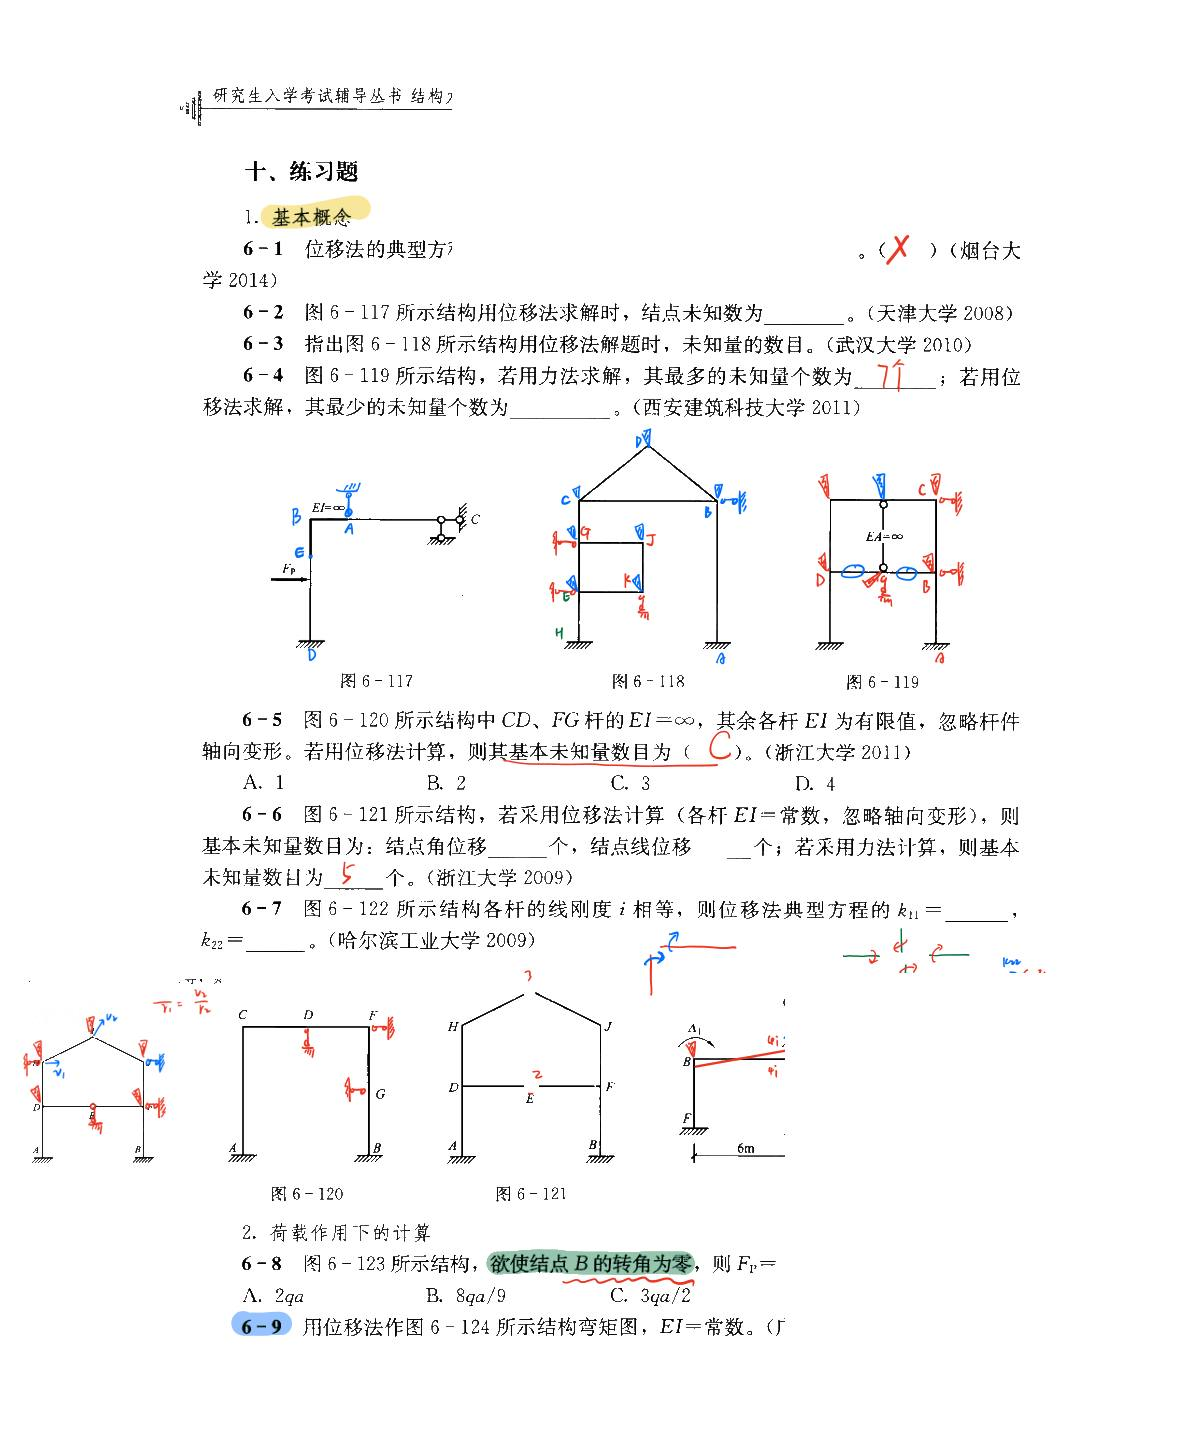
\includegraphics[width=0.92\textwidth]{figures/src31_p001.jpg}
\caption{【第11次作业笔记】 位移法(1) 第 1 页清理图形页}
\end{figure}
\subsection*{第 2 页转写}
6-10

用位移法作图6-125所示结构的弯矩图。（福州大学2011)

YXi+Rp=0

2E1

EI

图6-123

图6-124

Fp*

图6-125

Y"xit RP=D

Yas

Pp=元

213

XIMIt M:M

TuXit Yox++ Pp=o

o=de +Ex +iXnt

R.p= Fpl

2E1

2E1

661

EL

Rap=0

EI

EI

EI

EI

mp=0

2E1

139

二0

-6xi +i5X2=0
\begin{figure}[H]\centering
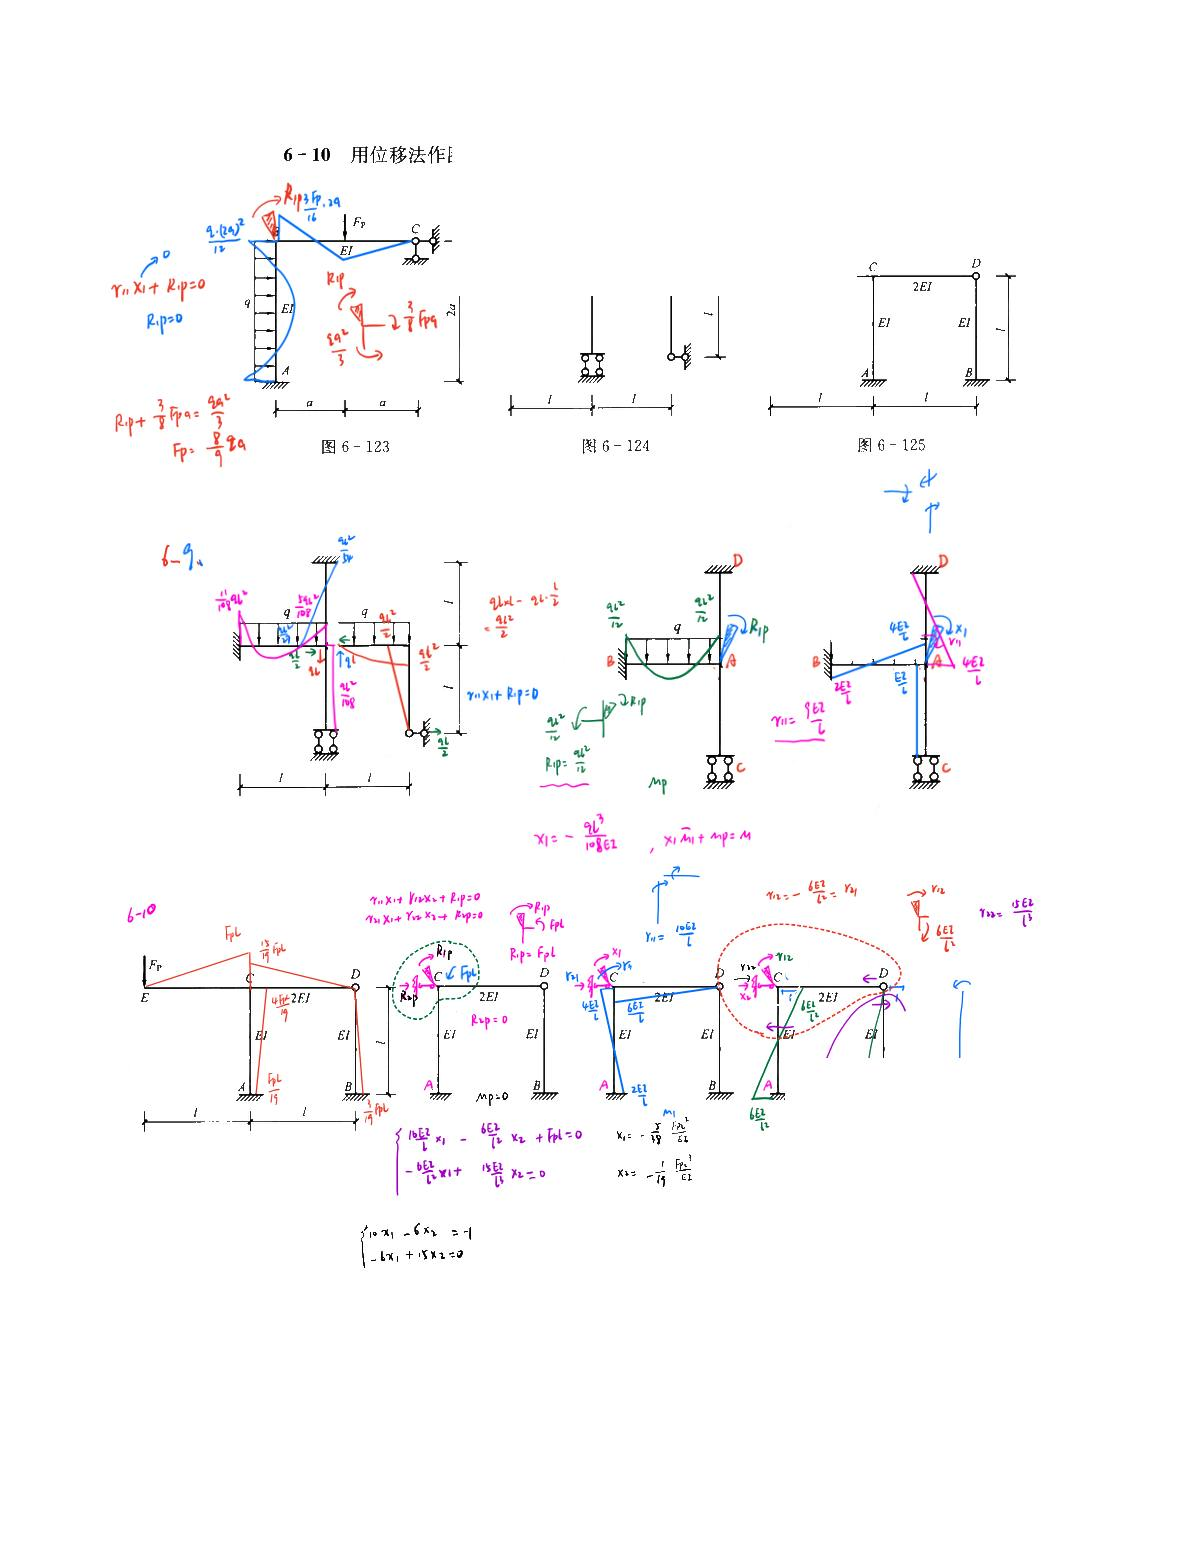
\includegraphics[width=0.92\textwidth]{figures/src31_p002.jpg}
\caption{【第11次作业笔记】 位移法(1) 第 2 页清理图形页}
\end{figure}
\subsection*{第 3 页转写}
6-11

用位移法计算图6－126所示结构，作其弯矩图。各受弯杆件EI=常数。（湖南

大学2011)

6-12

用位移法求图6-127所示无侧移刚架的杆端弯矩，并绘制弯矩图。设已知各杆

件的相对线刚度：横梁为1，竖柱为1.5。（中国地震局工程力学研究所2011）

60kN

21kN/m

150kNm

o=d +tx w +ix nt

1/2

1/2

12ml2ml

8m

图6-126

图6-127

Fp=ql

54t T

1/2

1/2

1/2

1/2

XI mItXi Mi+
\begin{figure}[H]\centering
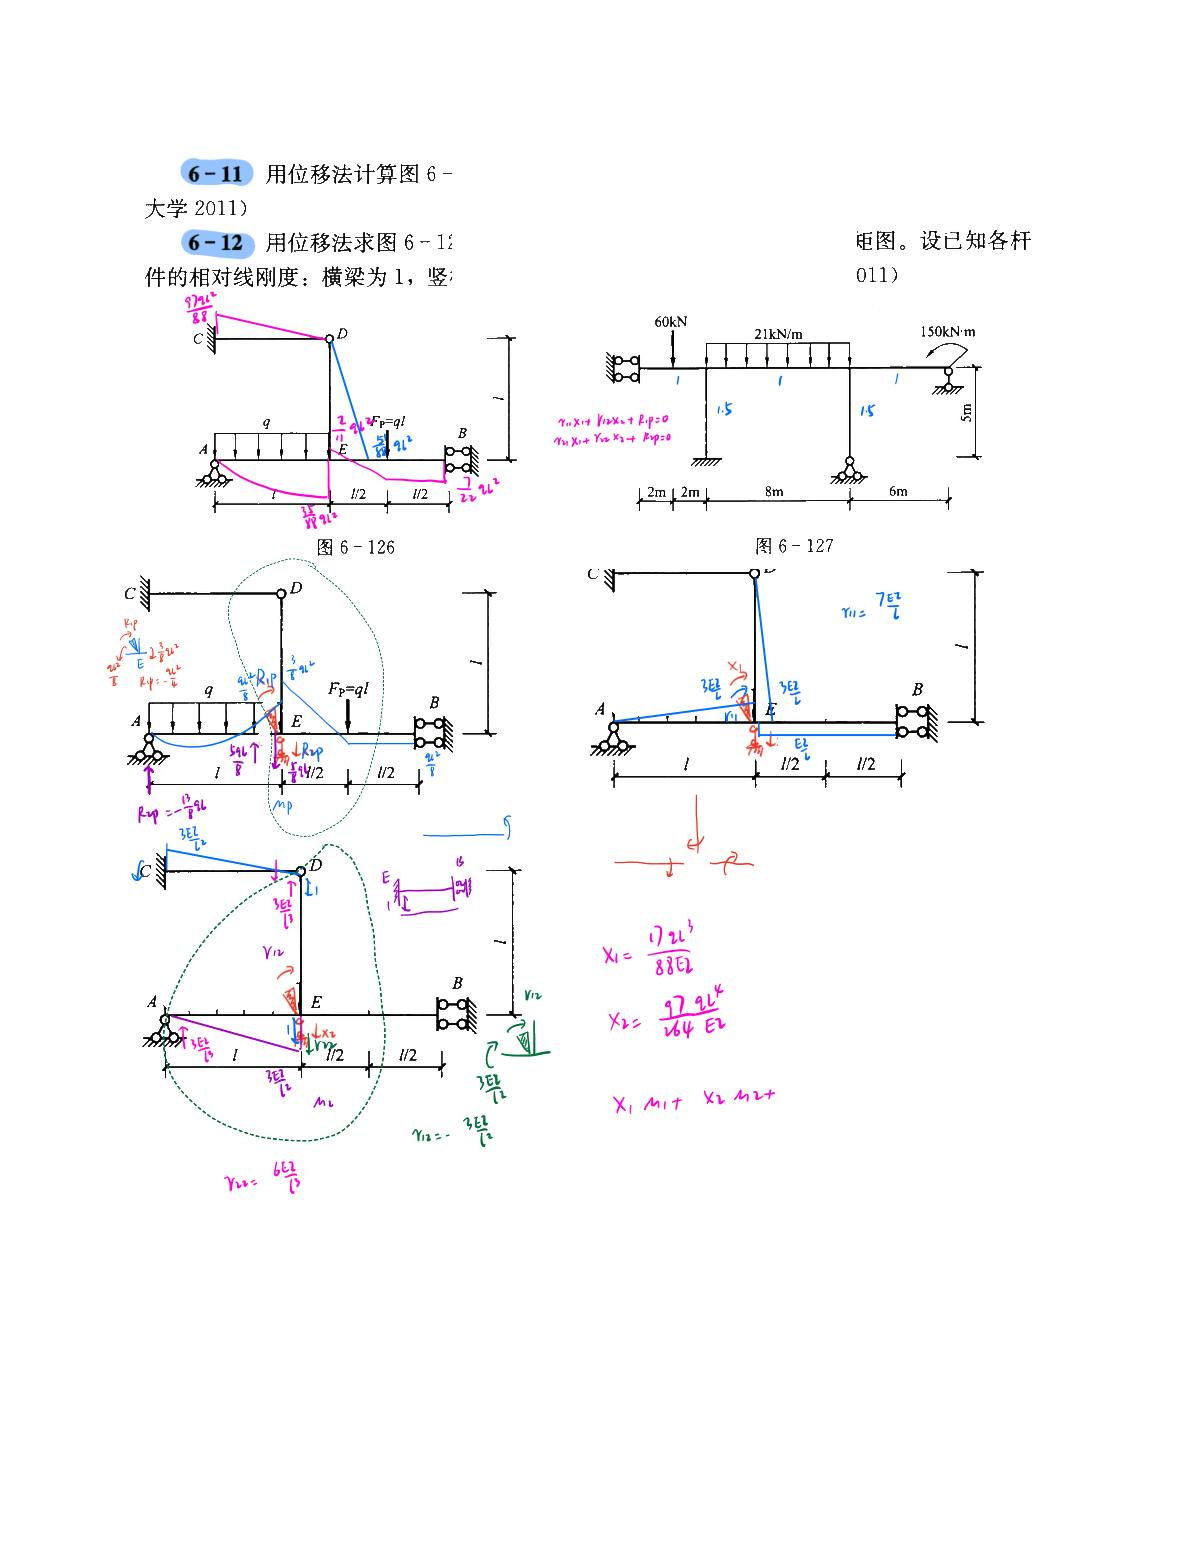
\includegraphics[width=0.92\textwidth]{figures/src31_p003.jpg}
\caption{【第11次作业笔记】 位移法(1) 第 3 页清理图形页}
\end{figure}
\subsection*{第 4 页转写}
60kN

21kN/m

150kN-m

XIe 2.6

X= -3.69

XIMI+

TXitYox-tPp=o

0=dd +txu +IXnt

8m

12m/2ml

6m

60kN

RIP

21kN/m

150kN-m

90

45

30

5m

8m

6m

12mj2m

12m/2ml

8m

6m

8m

12ml2m

6m
\begin{figure}[H]\centering
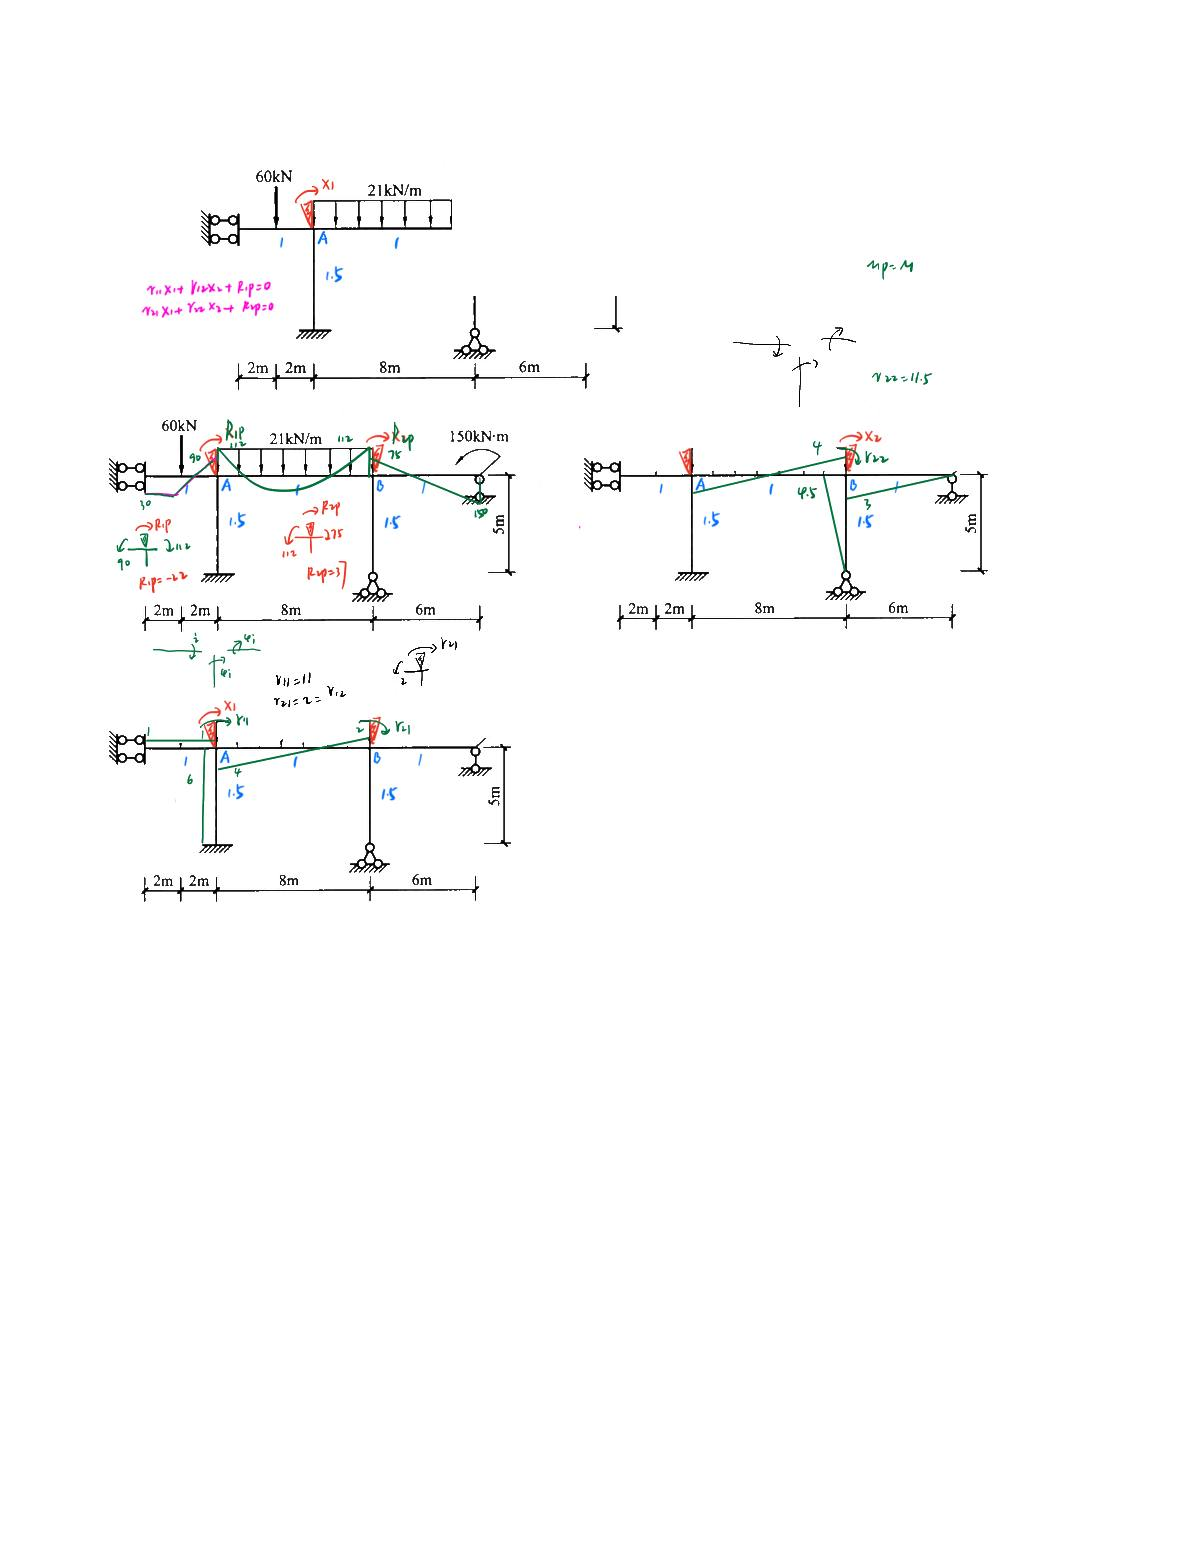
\includegraphics[width=0.92\textwidth]{figures/src31_p004.jpg}
\caption{【第11次作业笔记】 位移法(1) 第 4 页清理图形页}
\end{figure}
\subsection*{第 5 页转写}
用位移法求解图6－128所示结构，作M图。EI为常数。（青岛理工大学2010）

用位移法计算图6－129所示结构并作其弯矩图。（西安建筑科技大学2008）

1.5EI

34kN/m

3kN/m

2.24

16kNm

EL

3EI

455

EI

1.54

4m

5m

图6-128

图6-129

3.2

+ +"
\begin{figure}[H]\centering
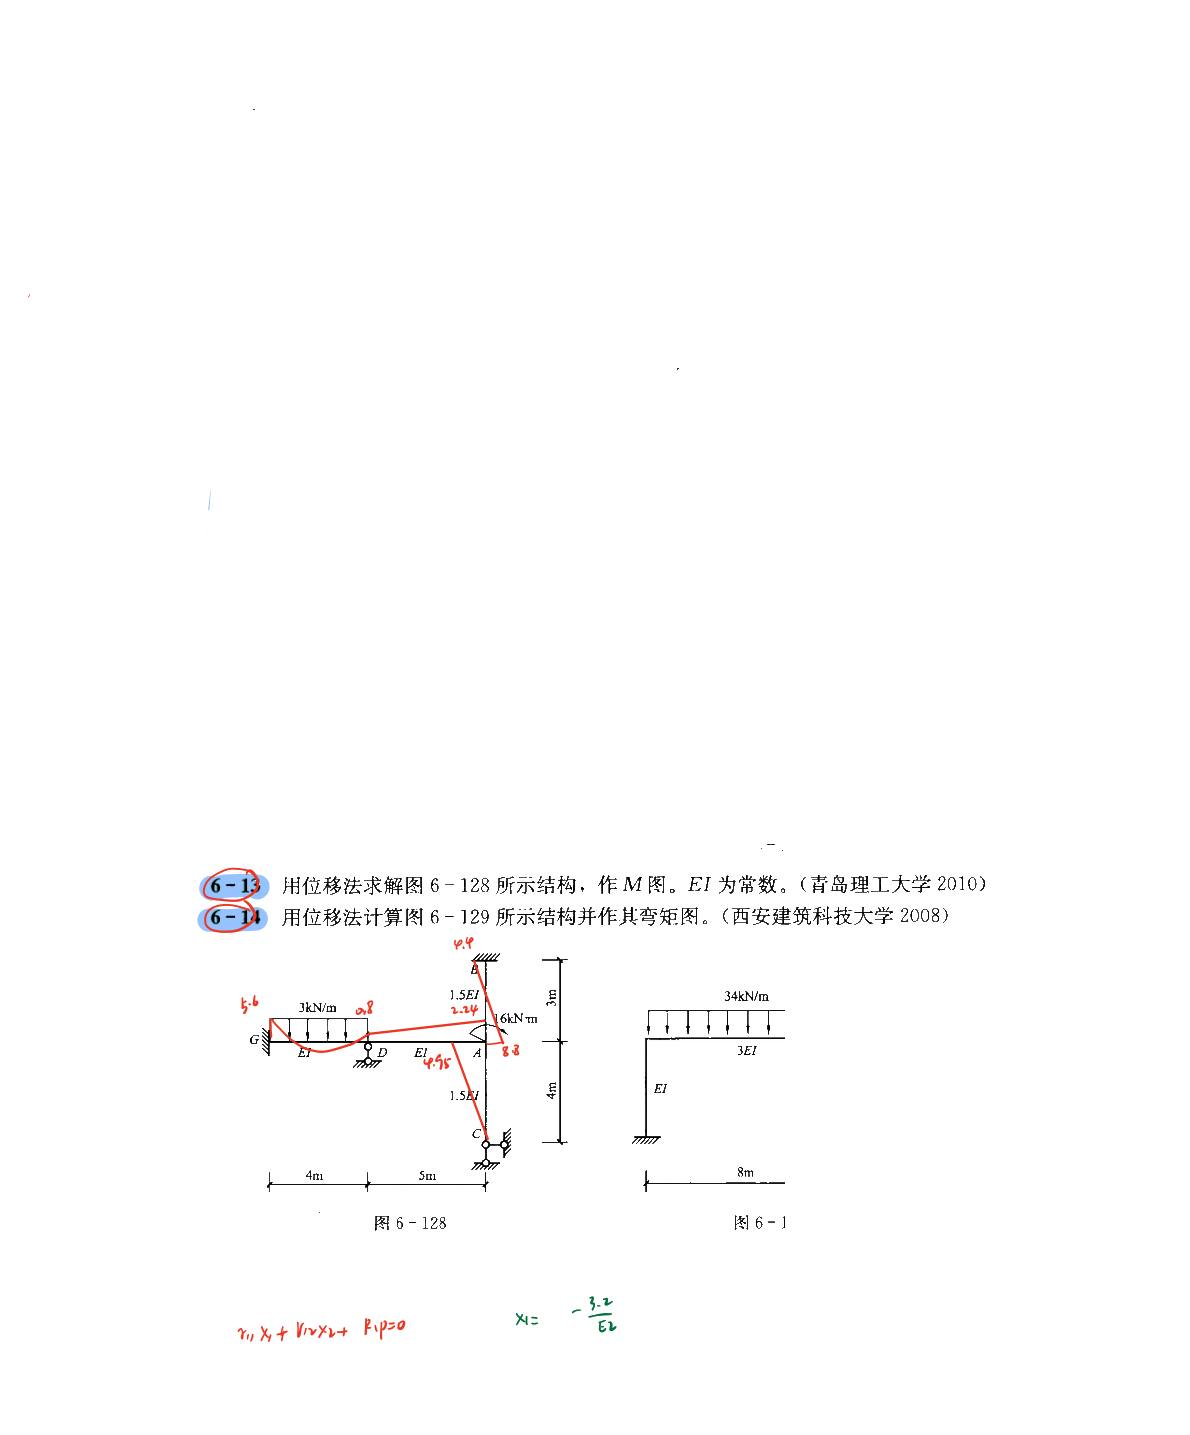
\includegraphics[width=0.92\textwidth]{figures/src31_p005.jpg}
\caption{【第11次作业笔记】 位移法(1) 第 5 页清理图形页}
\end{figure}
\subsection*{第 6 页转写}
1.5EI

3kN/m

16kNm

EI

1.5EI

1.5EI

4m

Rp=4

4m

5m

4m

797

PASEL

EI

3*15E2

1.5E

157

5m

4m

Y.xit p:0

34kN/m

3EL

4m

EI

13

8m

XI=

,XI mIt

34kN/m

EI

EI

8m

3.刚度无穷大杆件的计算

图6-130所示结构中截面A弯矩MA=

侧受拉。（哈尔滨工

业大学2011)

Y..X+ Rp-o

138

+iw'x
\begin{figure}[H]\centering
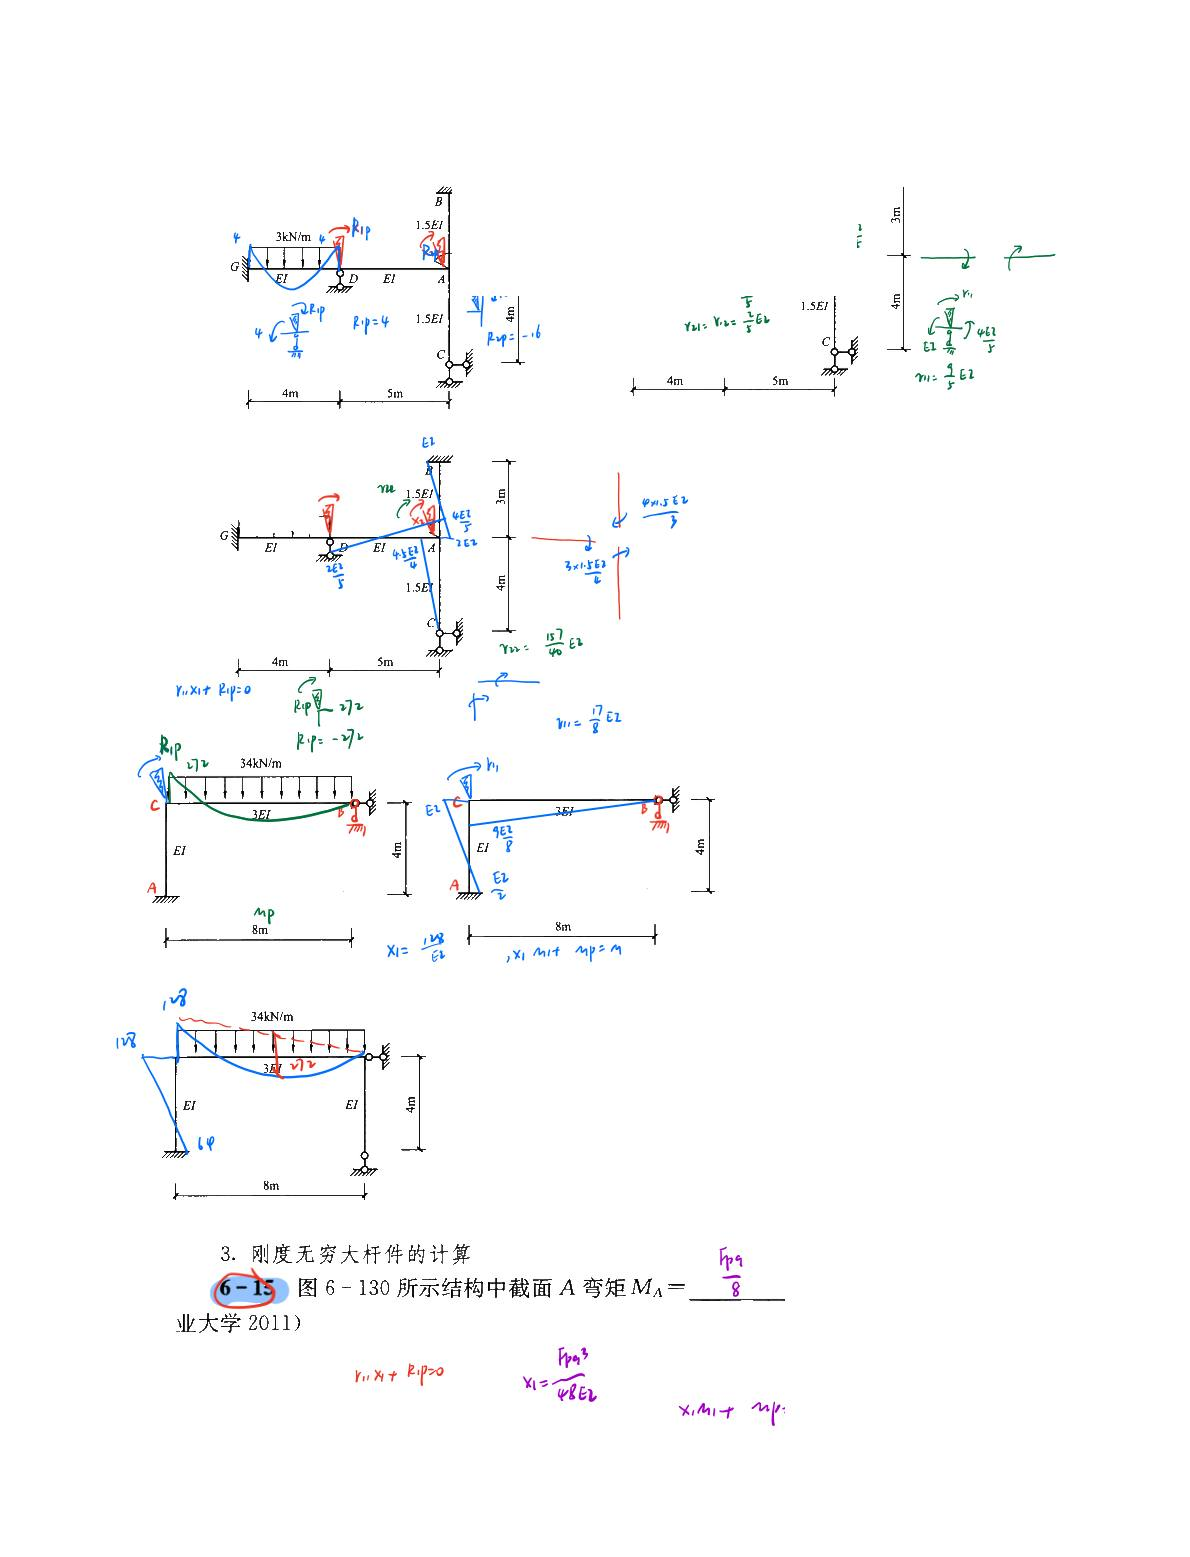
\includegraphics[width=0.92\textwidth]{figures/src31_p006.jpg}
\caption{【第11次作业笔记】 位移法(1) 第 6 页清理图形页}
\end{figure}
\subsection*{第 7 页转写}
El,=80

El,=00

El,=00

El,=00

Fp

EI

EI

Pp=-hp

El,=00

El,=00

EN

EA

EA

PIEL

ocdl +axu +IXxnn

b -16

fip- 24

12kN/m

12kN/m

Ele

EI

4m

El=00

EI

4m

4m

4m

4m

4m

4m

mp

X13

6EZ

14m

4m

64
\begin{figure}[H]\centering
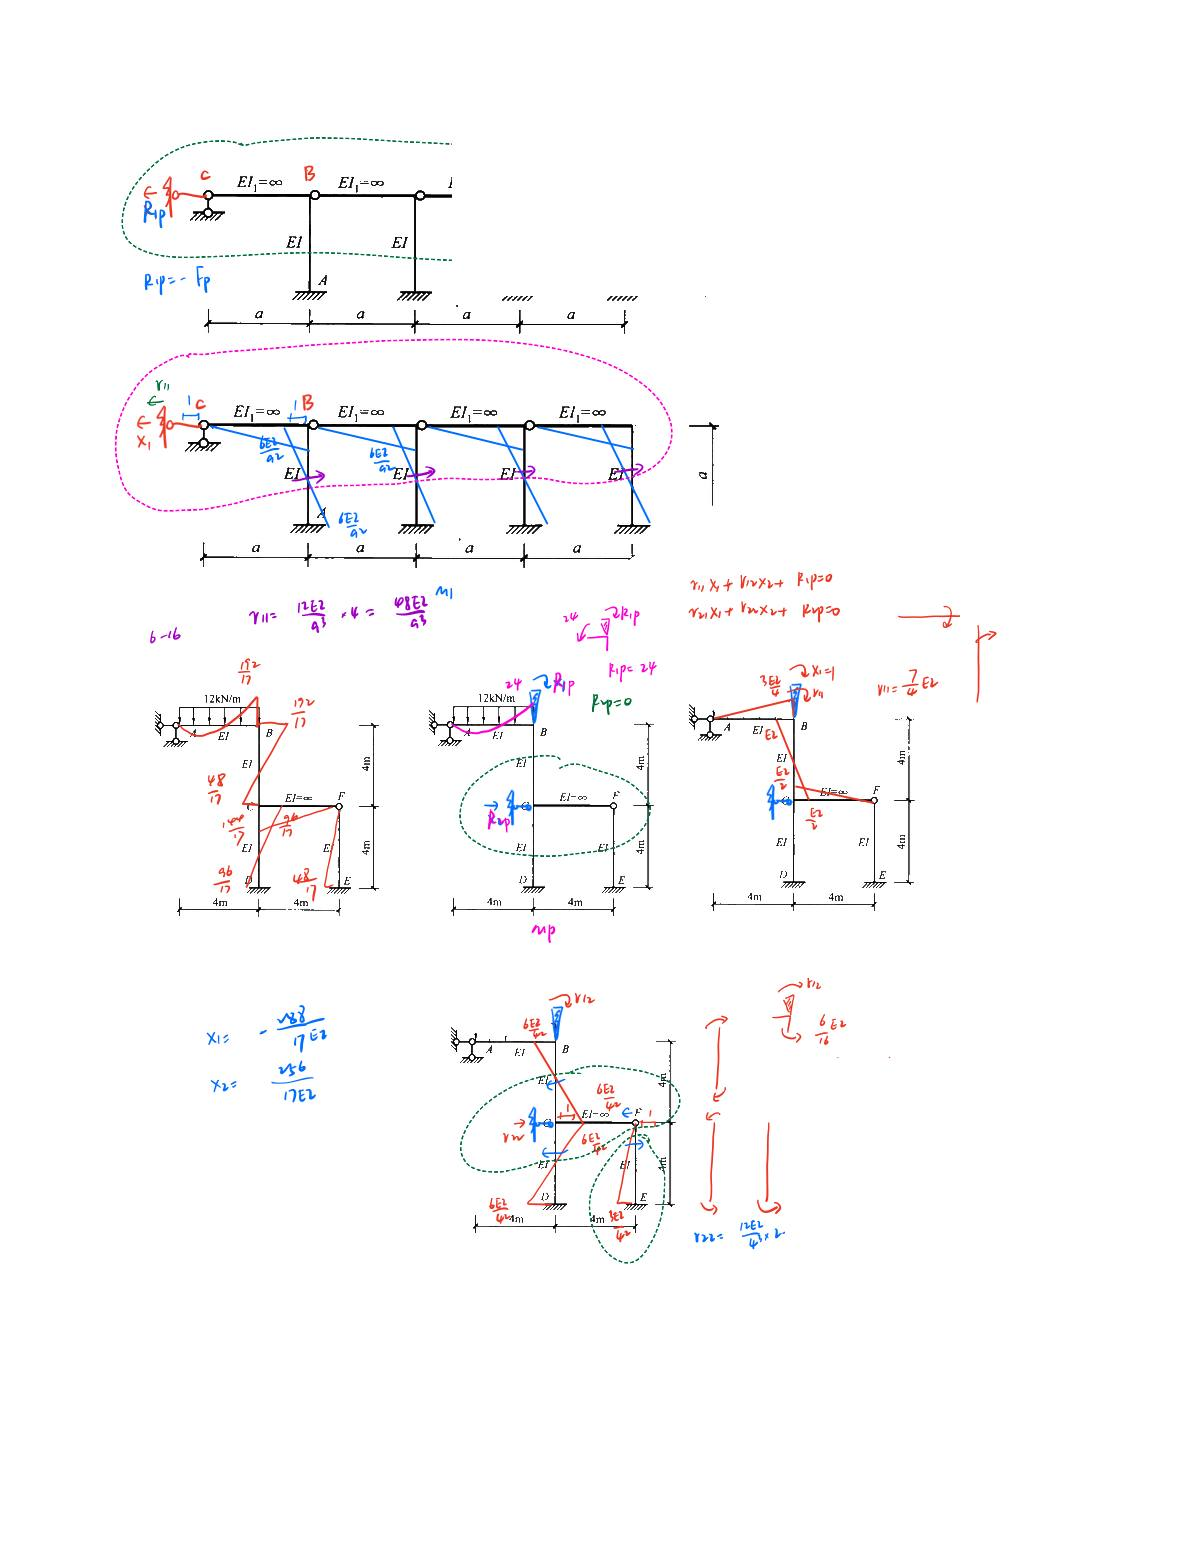
\includegraphics[width=0.92\textwidth]{figures/src31_p007.jpg}
\caption{【第11次作业笔记】 位移法(1) 第 7 页清理图形页}
\end{figure}
\subsection*{第 8 页转写}
6 - 17

作图6-132所示结构的M图、F。图及F\textasciitilde{}图。（中国矿业大学2009）

6 - 18

用位移法作图6-133所示结构的M图。设横梁EI为无限大，各柱相对线刚度

如图中所示。（华南理工大学2010）

EI

E1=00

EI

4kN/m

21

ID

图6-132

图6-133

Pip=-

El=00

EI

EI

TRP

, XIM1+ Mp:M

EI

15

AD, EA-00

BD, LA= 00,
\begin{figure}[H]\centering
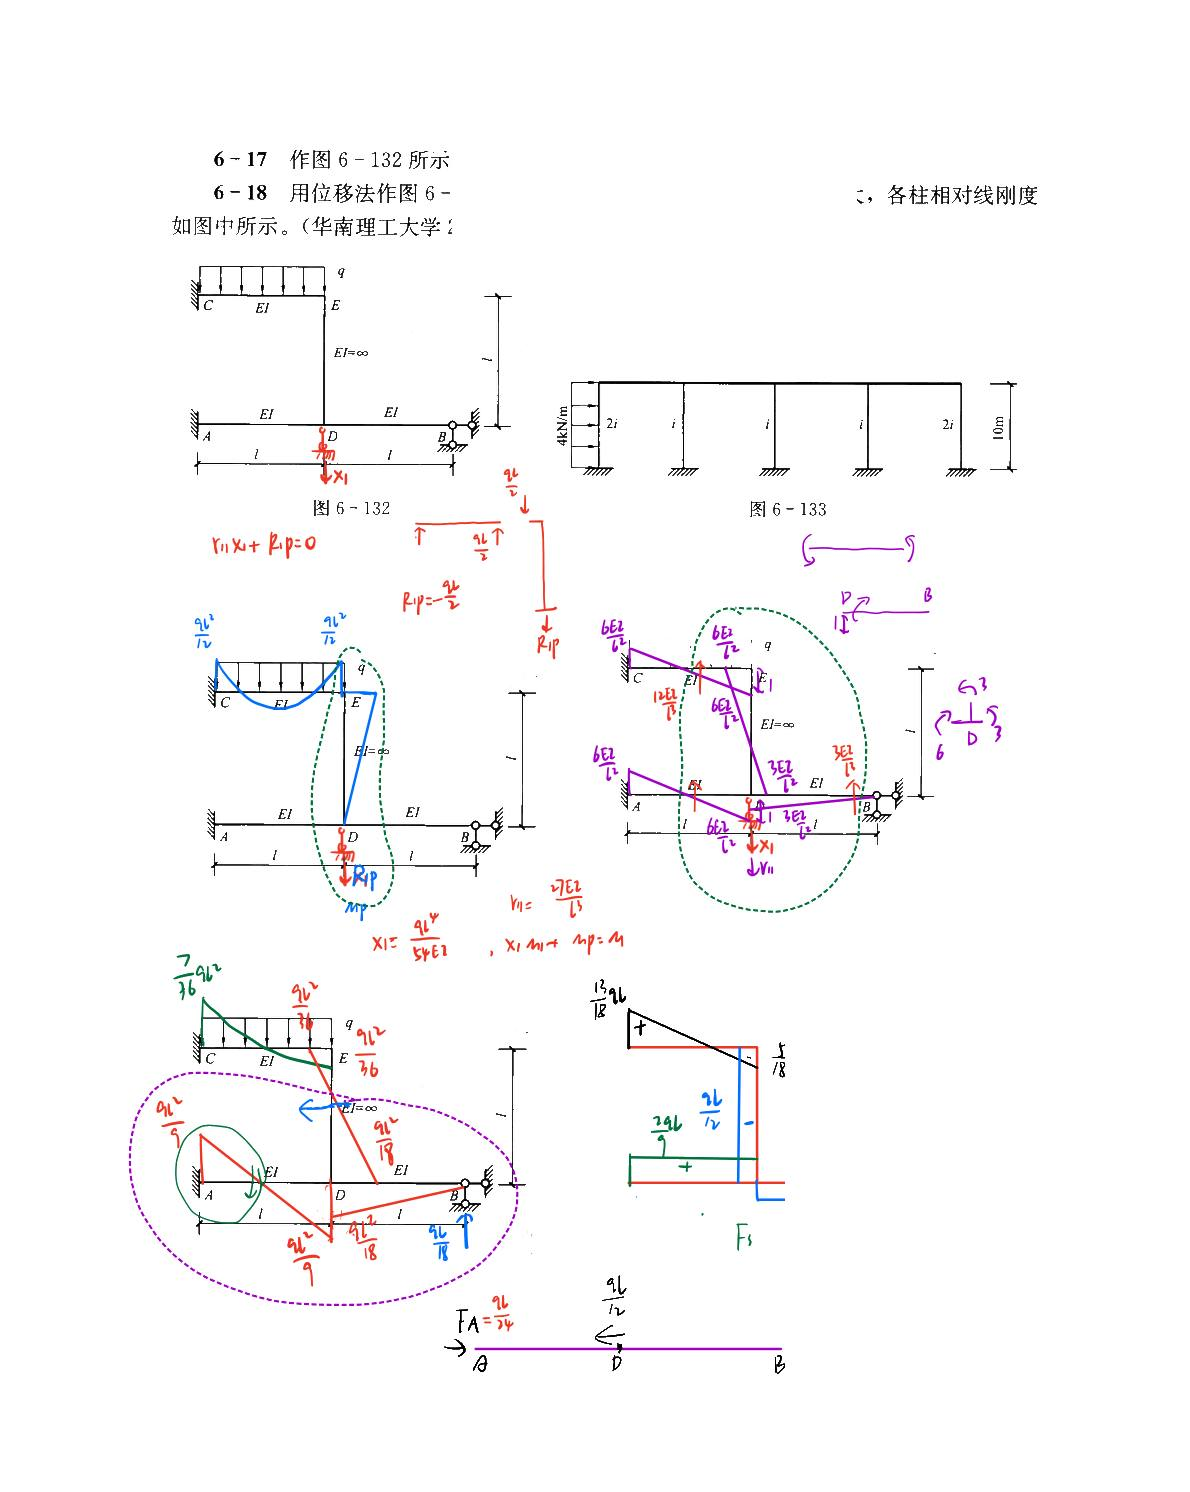
\includegraphics[width=0.92\textwidth]{figures/src31_p008.jpg}
\caption{【第11次作业笔记】 位移法(1) 第 8 页清理图形页}
\end{figure}
\subsection*{第 9 页转写}
注意：杆件变形量为 ，杆轴力为

贰心

 

  gi 

Qcxl 三i tilx  tiqi

Ocjal

jail

Qc i9L

it

E

1

i

l D

i

i

i

i

 

 

毕

AEF

Fit Fr Fp

EAh.li

筑

一筑

主忄 

A

兵El籪

靠

E

D

C

B

Ao\_o

7x

rnXit Rip0

可

41

1，02

在

in iii

Rip

20

iiiiiiiW.iiiii.i m
\begin{figure}[H]\centering
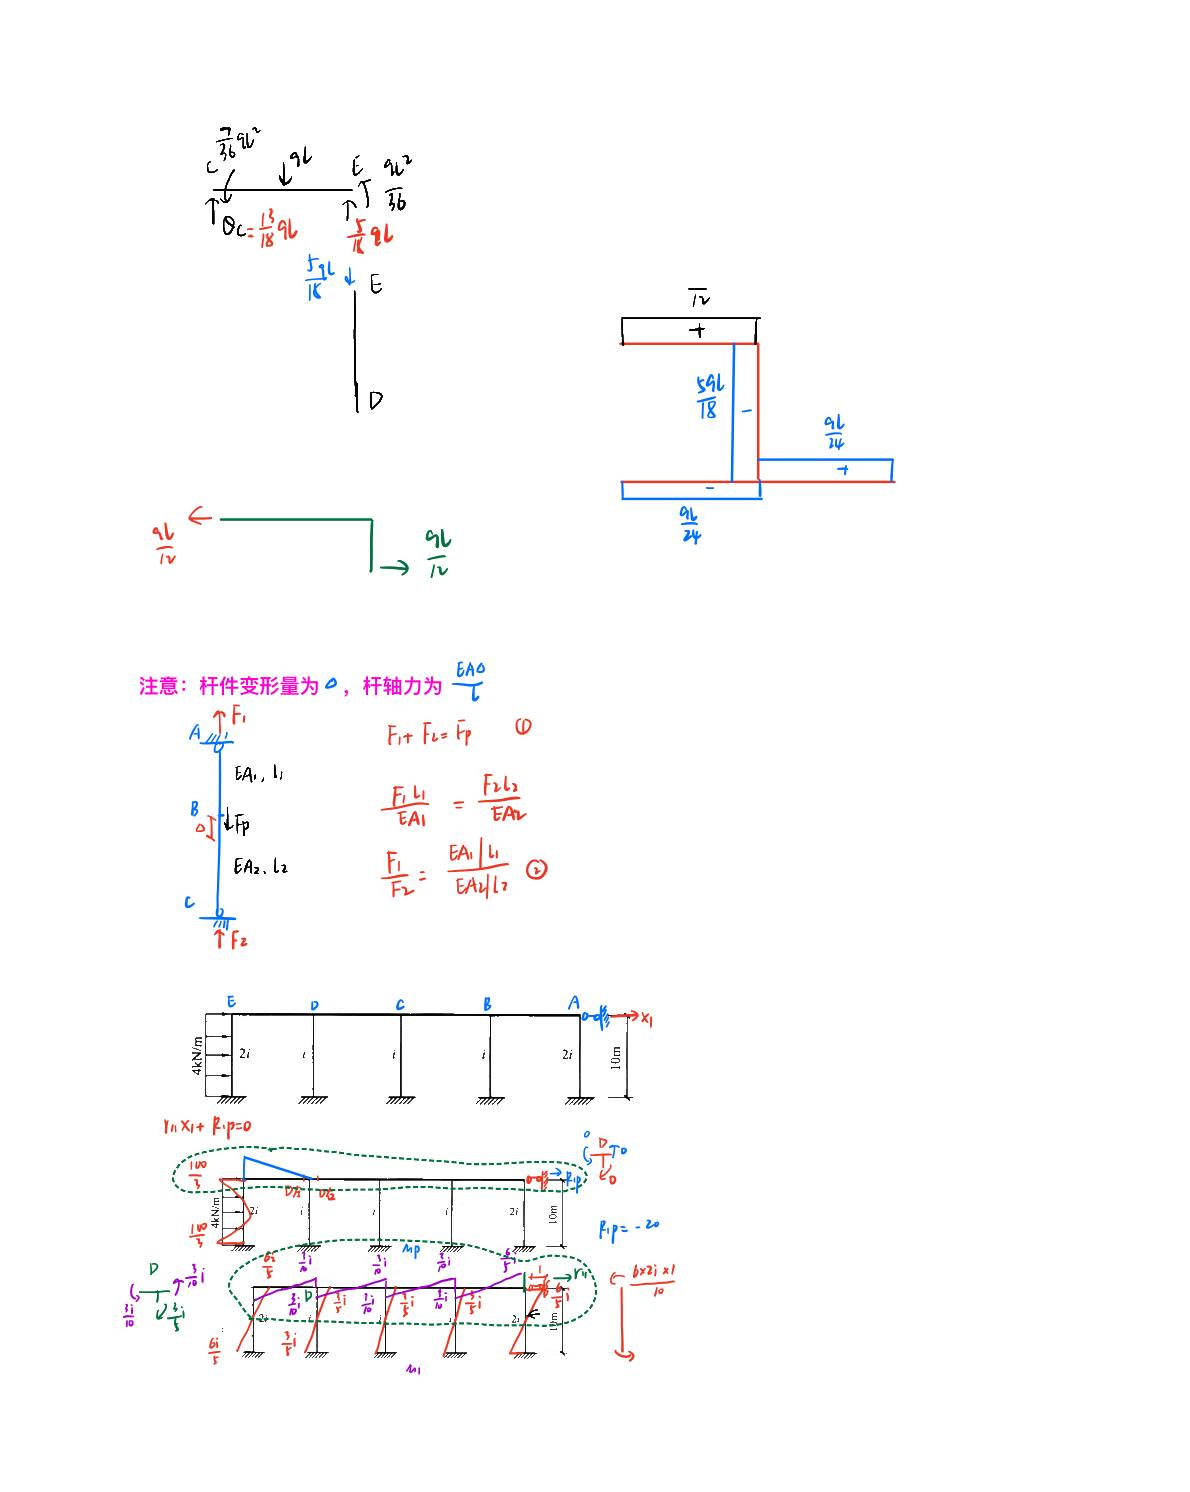
\includegraphics[width=0.92\textwidth]{figures/src31_p009.jpg}
\caption{【第11次作业笔记】 位移法(1) 第 9 页清理图形页}
\end{figure}
\subsection*{第 10 页转写}
1

1

1

i Rip

Xi二器

te 等i x2 器亢心了等

xim.tnp M

i

 

iiyiii

2

些

i

竿

nlkn.in
\begin{figure}[H]\centering
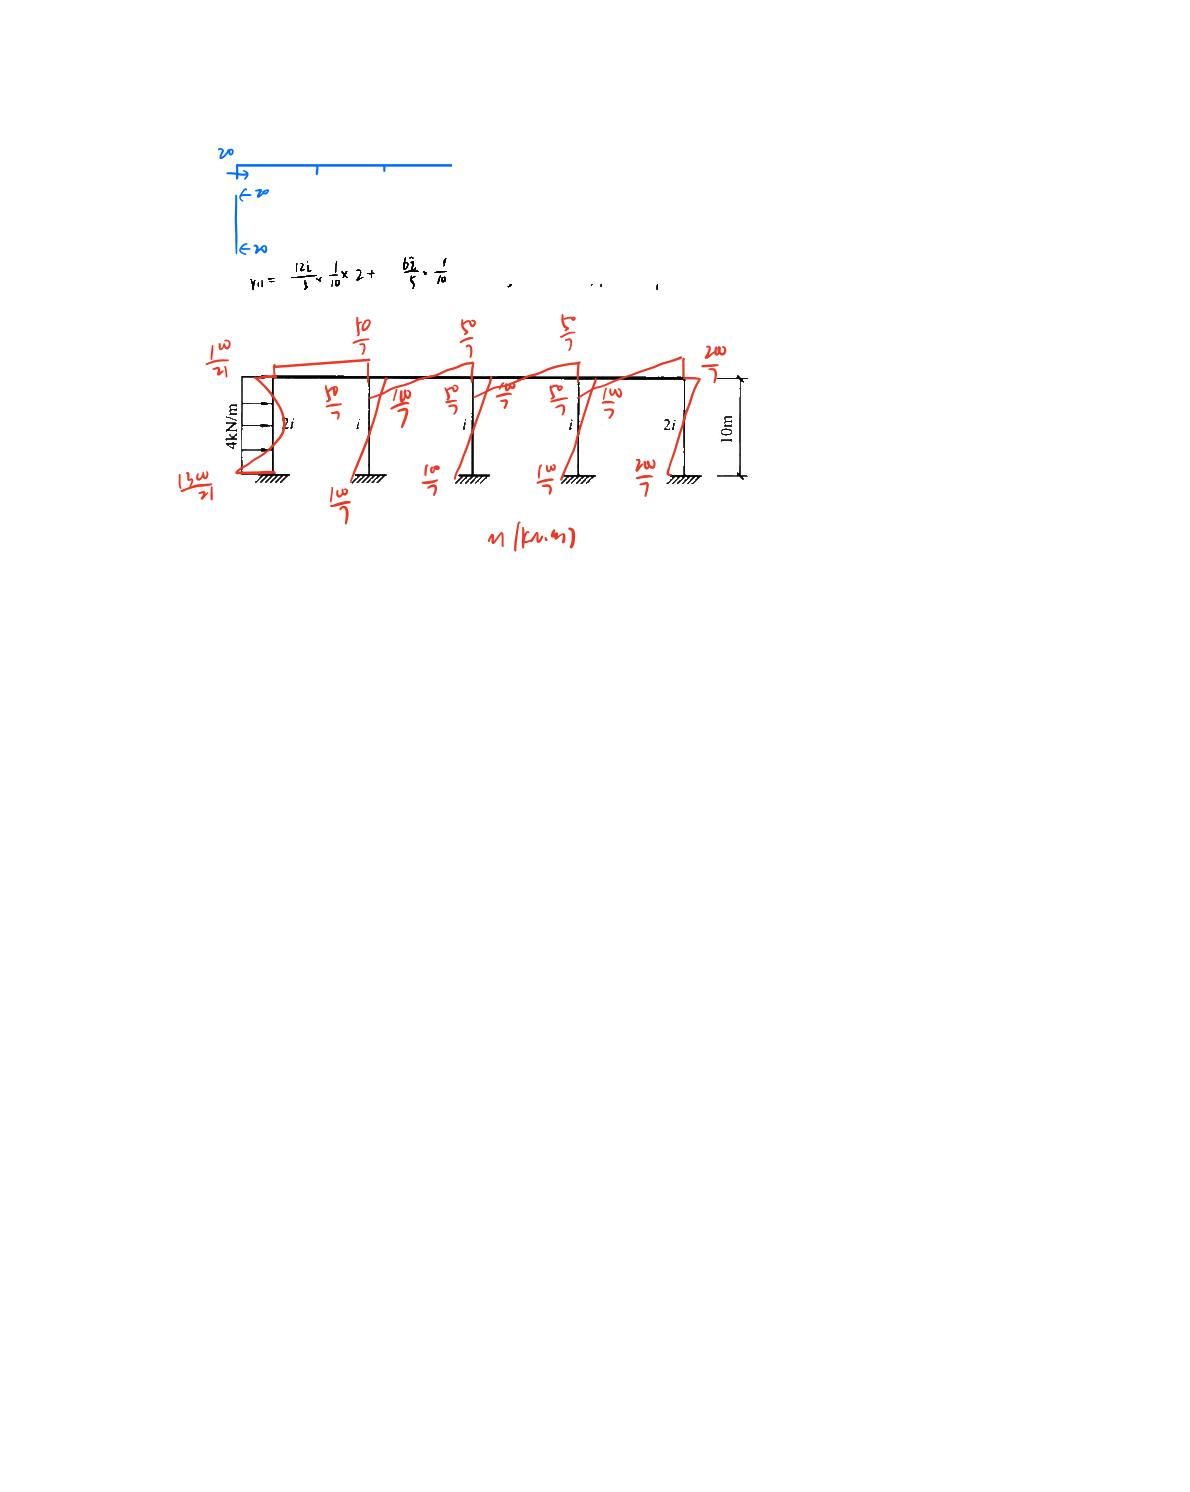
\includegraphics[width=0.92\textwidth]{figures/src31_p010.jpg}
\caption{【第11次作业笔记】 位移法(1) 第 10 页清理图形页}
\end{figure}
\subsection*{第 11 页转写}
6-19

用位移法求图6－134所示结构的弯矩图。EI=常数。（北京工业大学2013）

6-20

用位移法作图6-135所示结构弯矩图。EI=常数。（苏州科技学院2007、华南

理工大学2006)

图6-134

图6-135\%

Y..Xit R.p=0

308

Rip= -
\begin{figure}[H]\centering
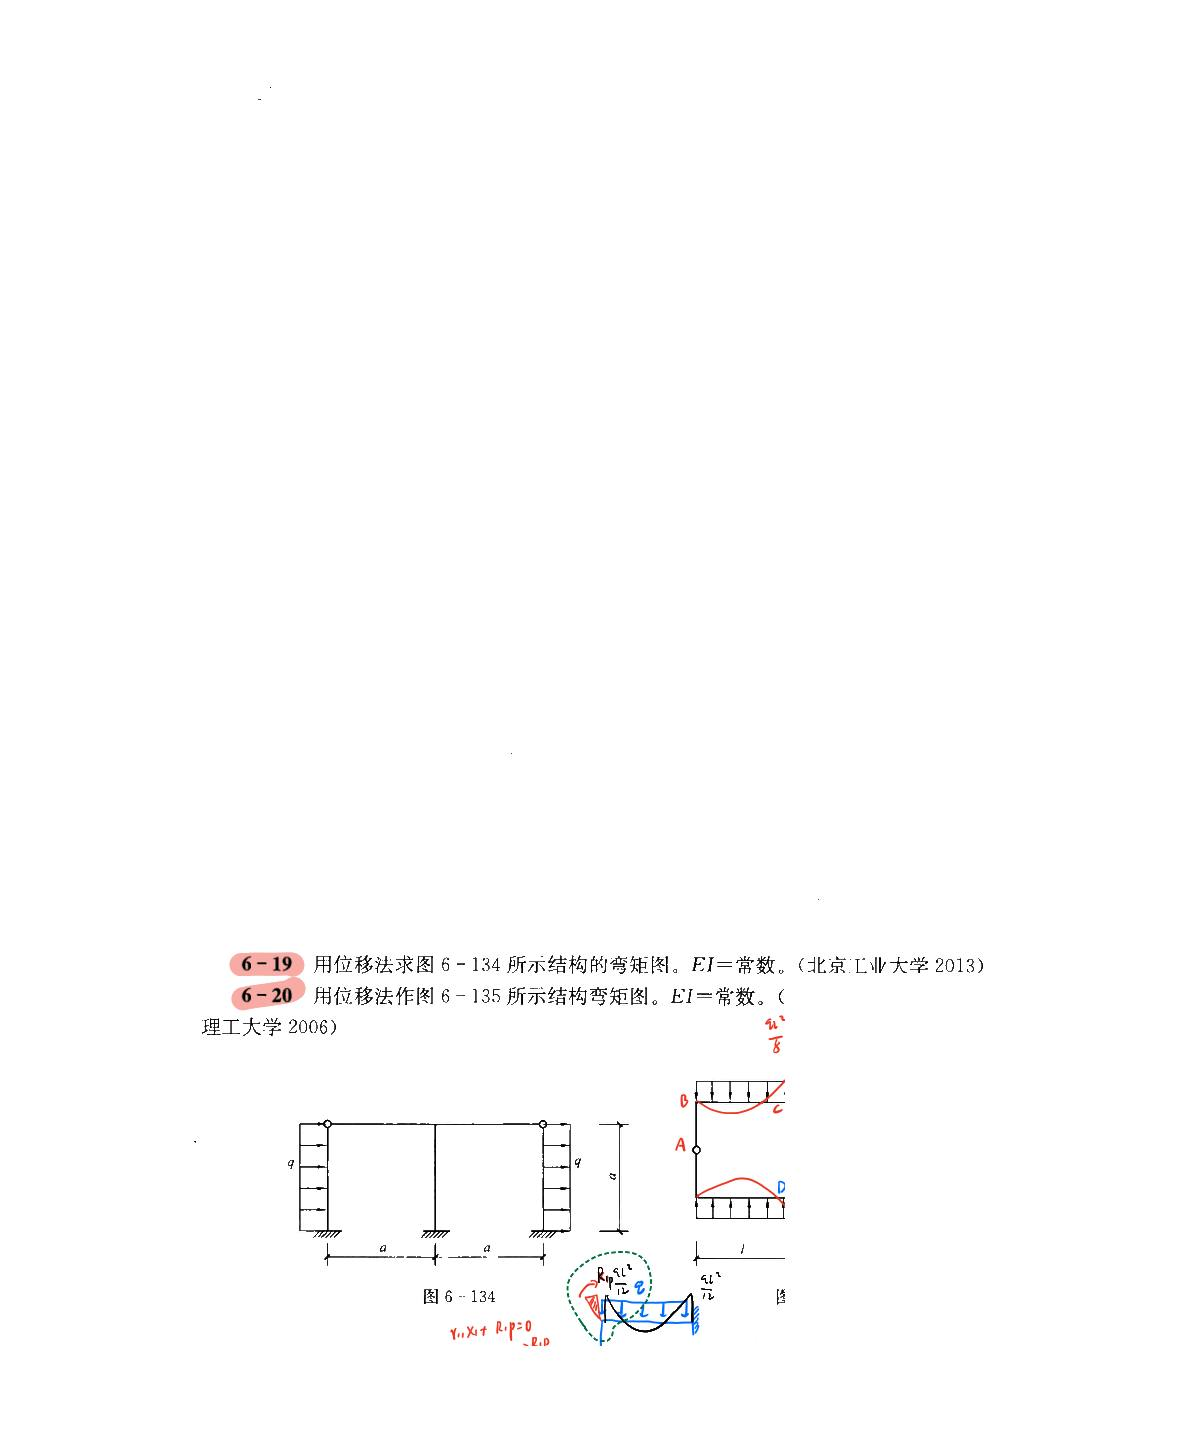
\includegraphics[width=0.92\textwidth]{figures/src31_p011.jpg}
\caption{【第11次作业笔记】 位移法(1) 第 11 页清理图形页}
\end{figure}
\subsection*{第 12 页转写}
Rpt

P=0

+Ix以

XIMI+

6-21

作图6-136所示结构的M图，各杆EI=常数。（西南交通大学2010）

6 - 22

用位移法作图6-137所示结构M图。各杆EI=常数。（山东建筑大学2012）

3.5

4kN/m

21

21

3m

3m

1/2

1/2

图6-136

图6-137
\begin{figure}[H]\centering
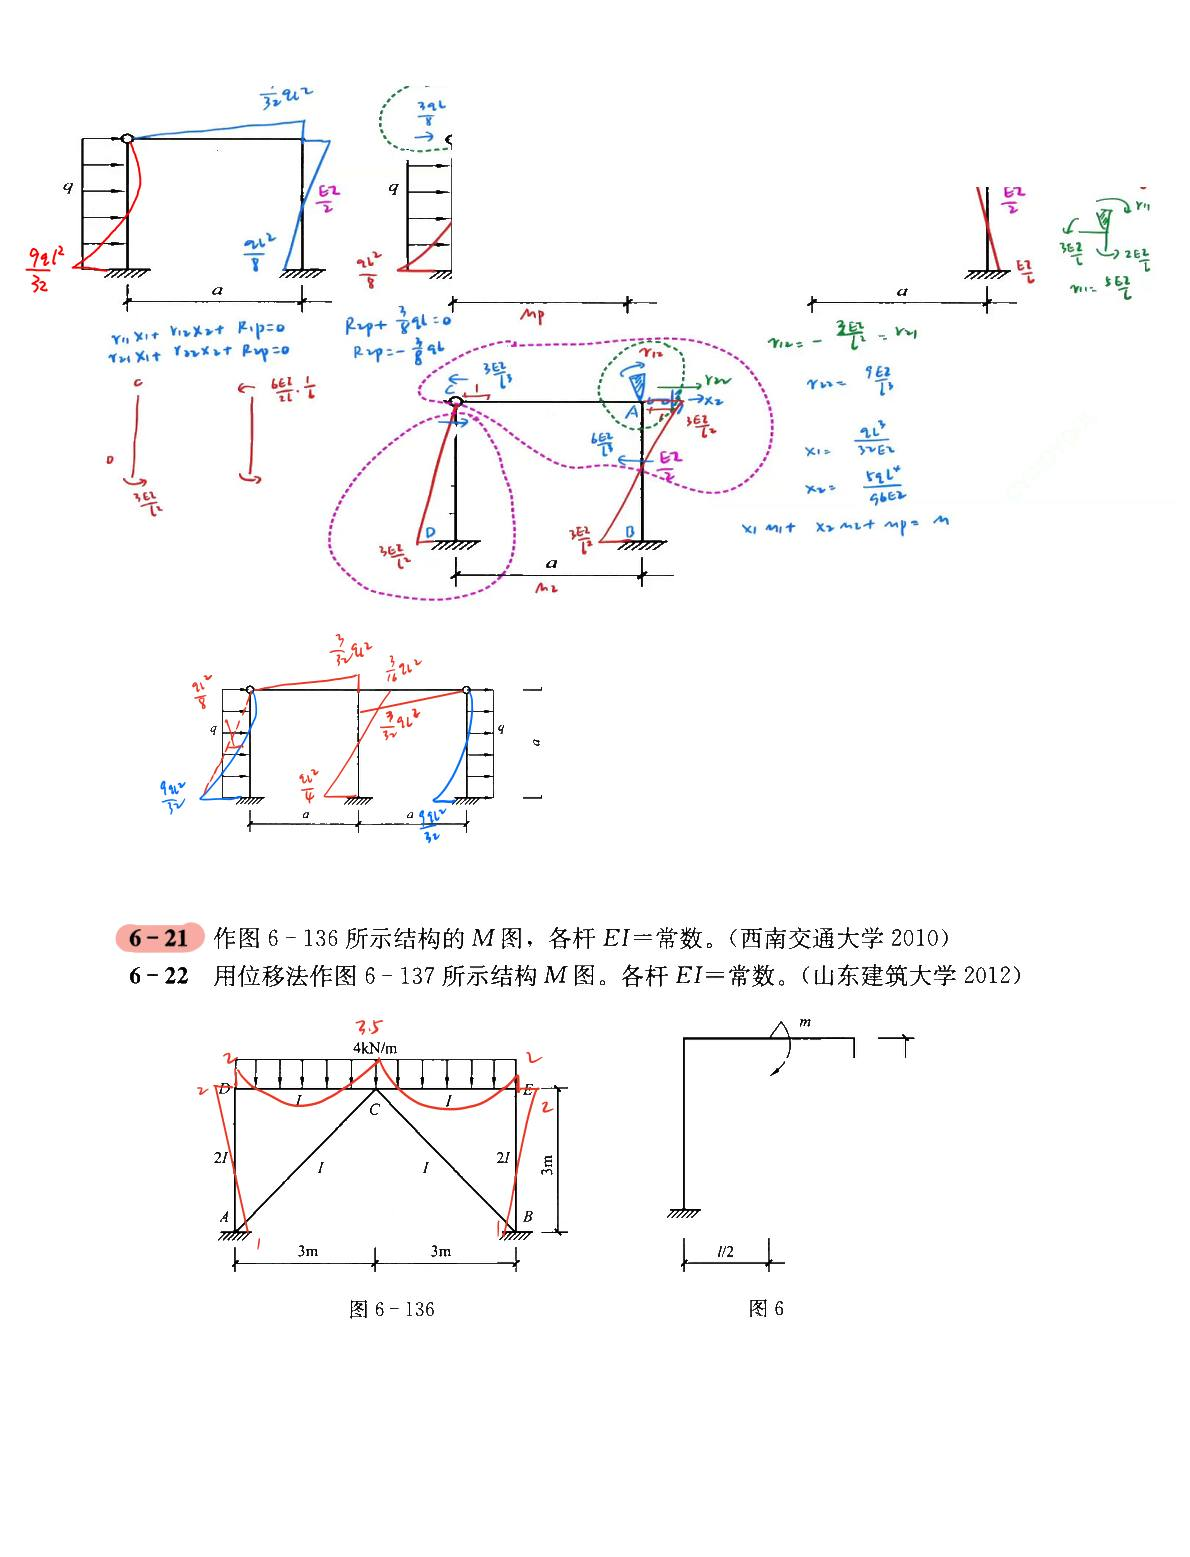
\includegraphics[width=0.92\textwidth]{figures/src31_p012.jpg}
\caption{【第11次作业笔记】 位移法(1) 第 12 页清理图形页}
\end{figure}
\subsection*{第 13 页转写}
Yuxt Kpo

2.S 4kN/m

4kN/m

YEL

21

3m

3m

3m

X13

Xi MI+ mp: M

1/2

1/2

TEL

XiMItmp:M

6-23用位移法作图6-138所示结构M图。各杆EI=常数。（山东建筑大学2009）

6-24

用位移法作图6-139所示结构M图。已知各杆EI=常数。（广西大学2010年）

40kN

1/2

4m

/2

2m-

4m

.xit R.pzo

图6-139

图6-138
\begin{figure}[H]\centering
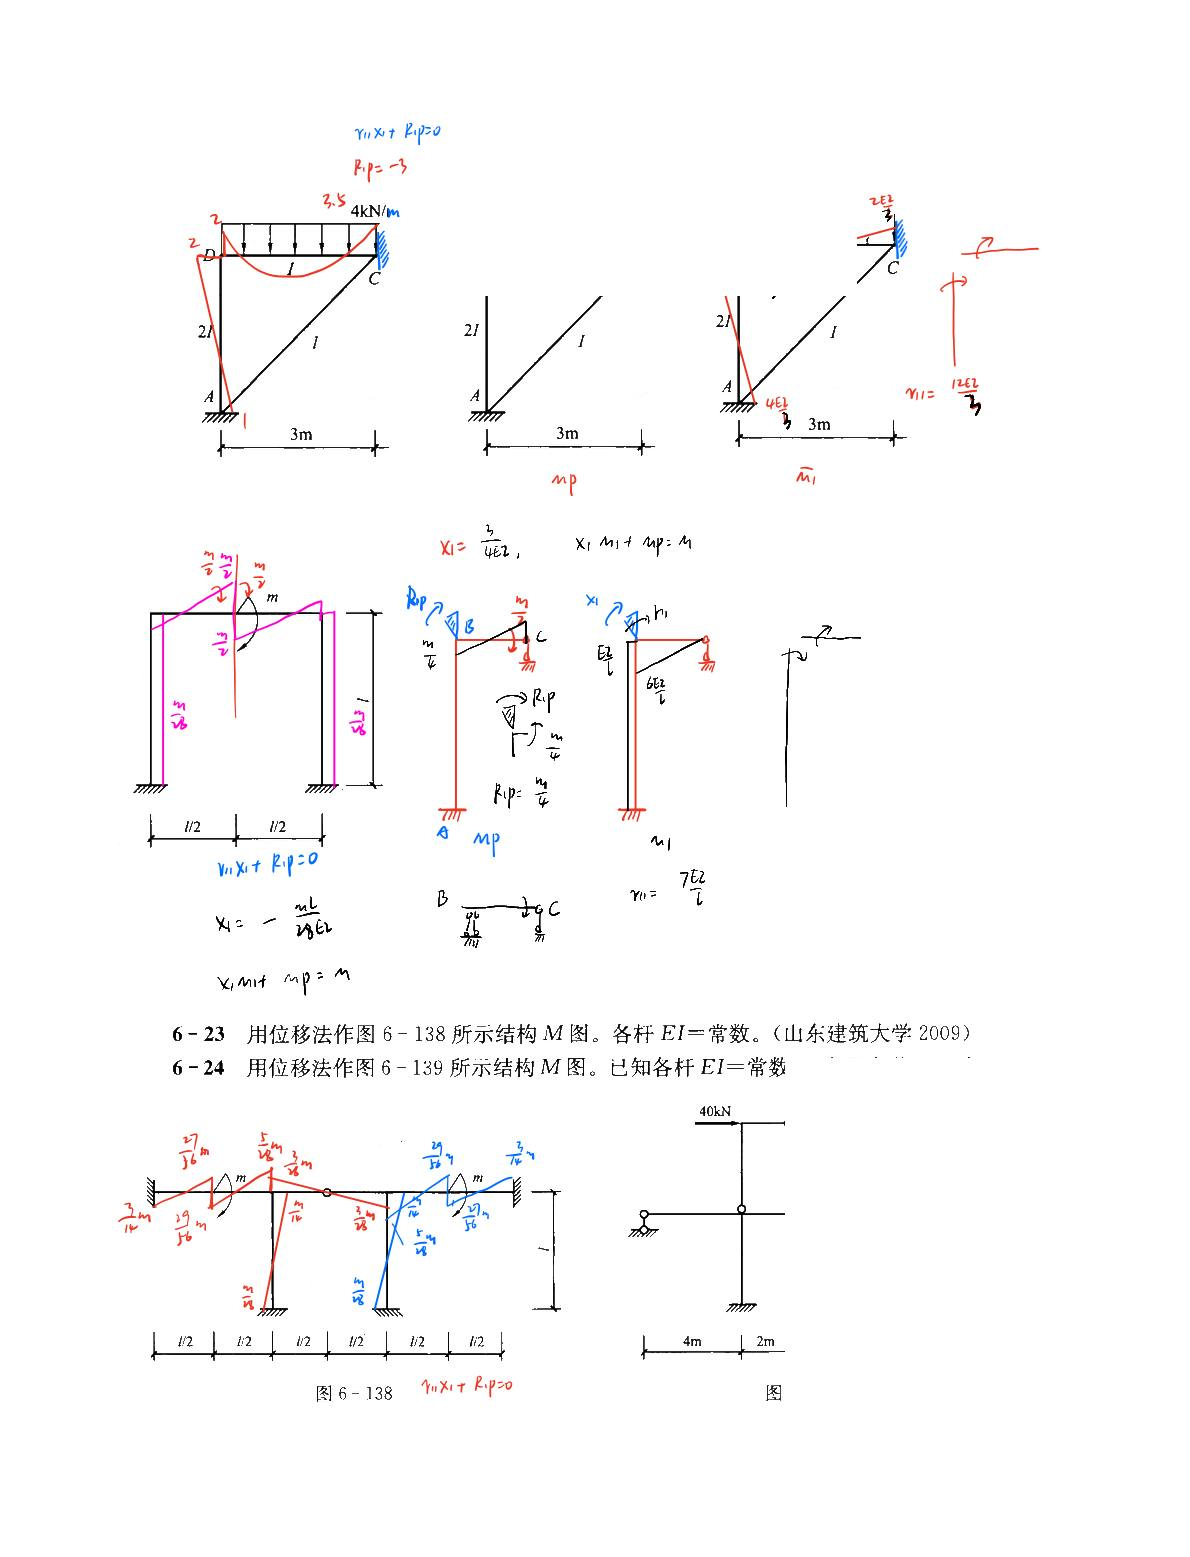
\includegraphics[width=0.92\textwidth]{figures/src31_p013.jpg}
\caption{【第11次作业笔记】 位移法(1) 第 13 页清理图形页}
\end{figure}
\subsection*{第 14 页转写}
XI MI+ mP: M

1/2

1/2

1/2

1/2

1/2

1/2

1/2

1/2

1/2

70 KN

24

4m

4m

4m

2m

2m

Rpe-to

2m

4m

4m

2m

mp

XI mi+ mp= M
\begin{figure}[H]\centering
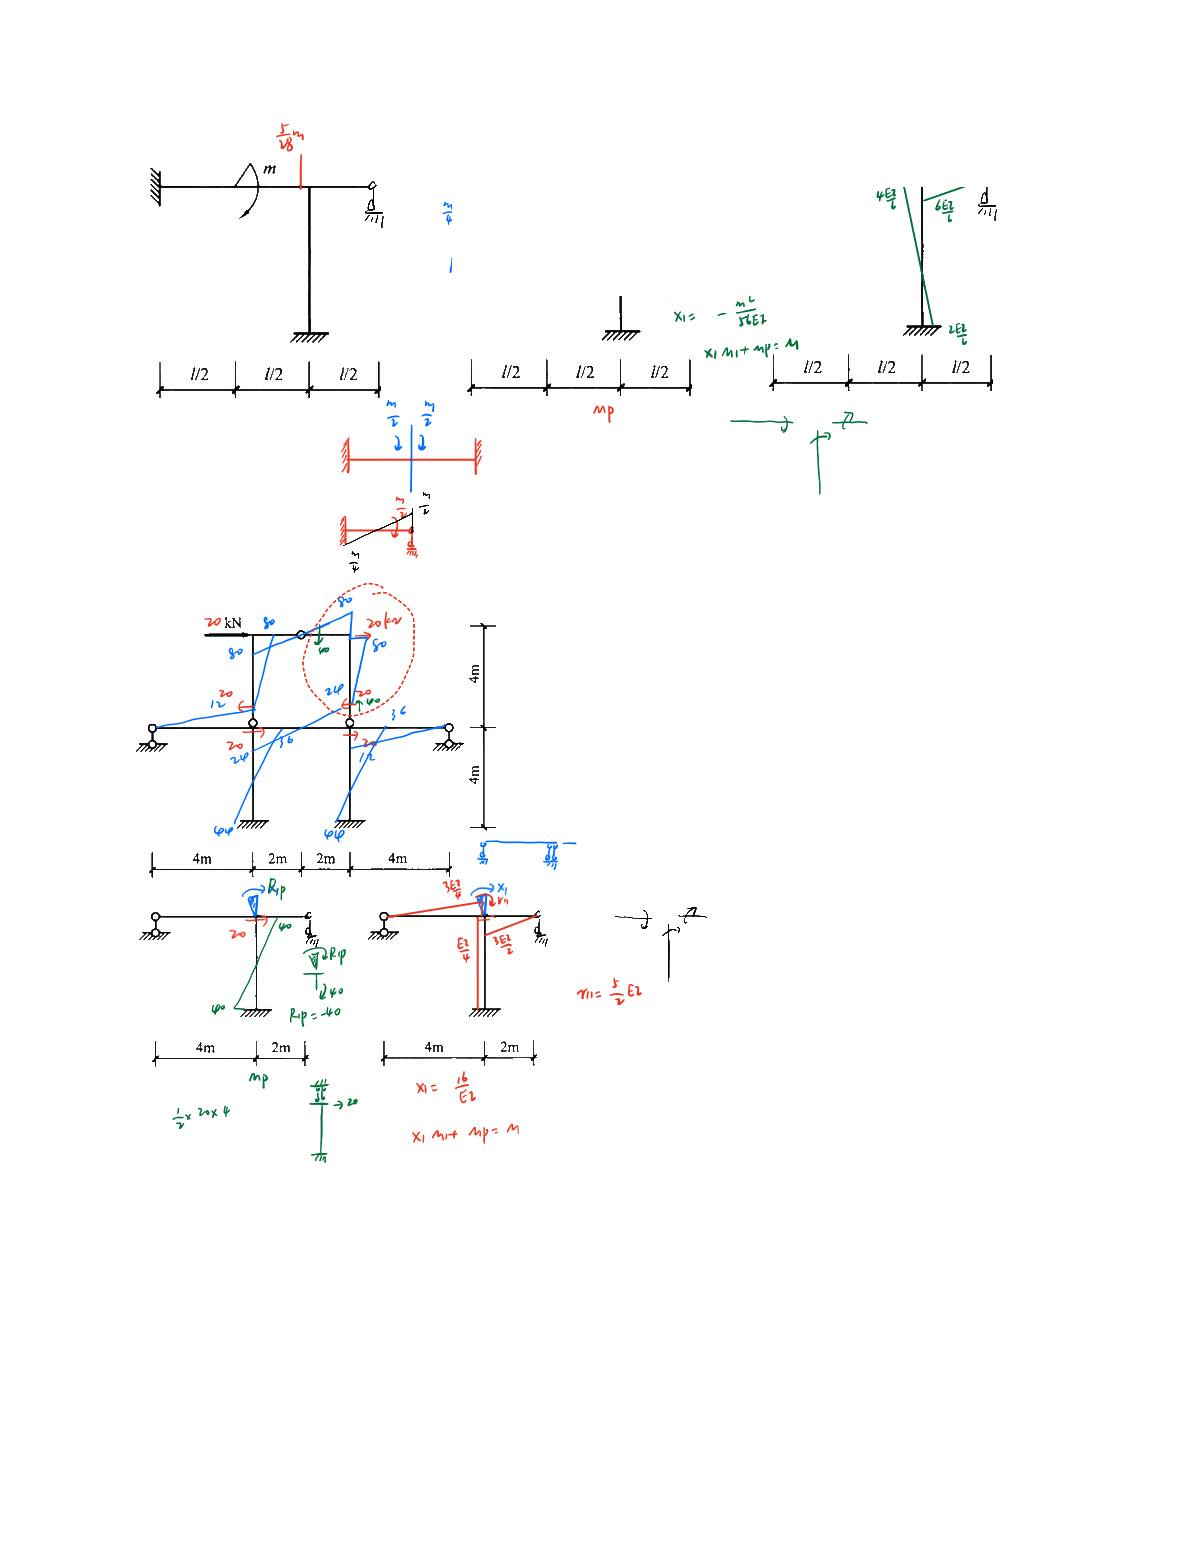
\includegraphics[width=0.92\textwidth]{figures/src31_p014.jpg}
\caption{【第11次作业笔记】 位移法(1) 第 14 页清理图形页}
\end{figure}
\subsection*{第 15 页转写}
6-25用合适的方法计算图6-140所示对称结构，并作出M图。EI=常数。（中国矿

业大学2011)

6-26

根据对称性用位移法求解图6-141所示结构，作M图。EI为常数。（青岛理工

大学2012)

12kN

3kN/m

EI

JkN/m

EI

EI

6m

6m

4m

4m

2m

2m

4m

4m

图6-140

1A1

12k

3kN/m

0.56

1.204

6m

0.60

XI:

2m

4m

400

4m

bKN

3kN/m

3.34

1131

EI

6m

6m

0.00

12m

2m

4m

4m

4m

2m

2m

4m

EI

Rip= 05

2m

2m

2m

2m

2m

2m

XiMit Mpem
\begin{figure}[H]\centering
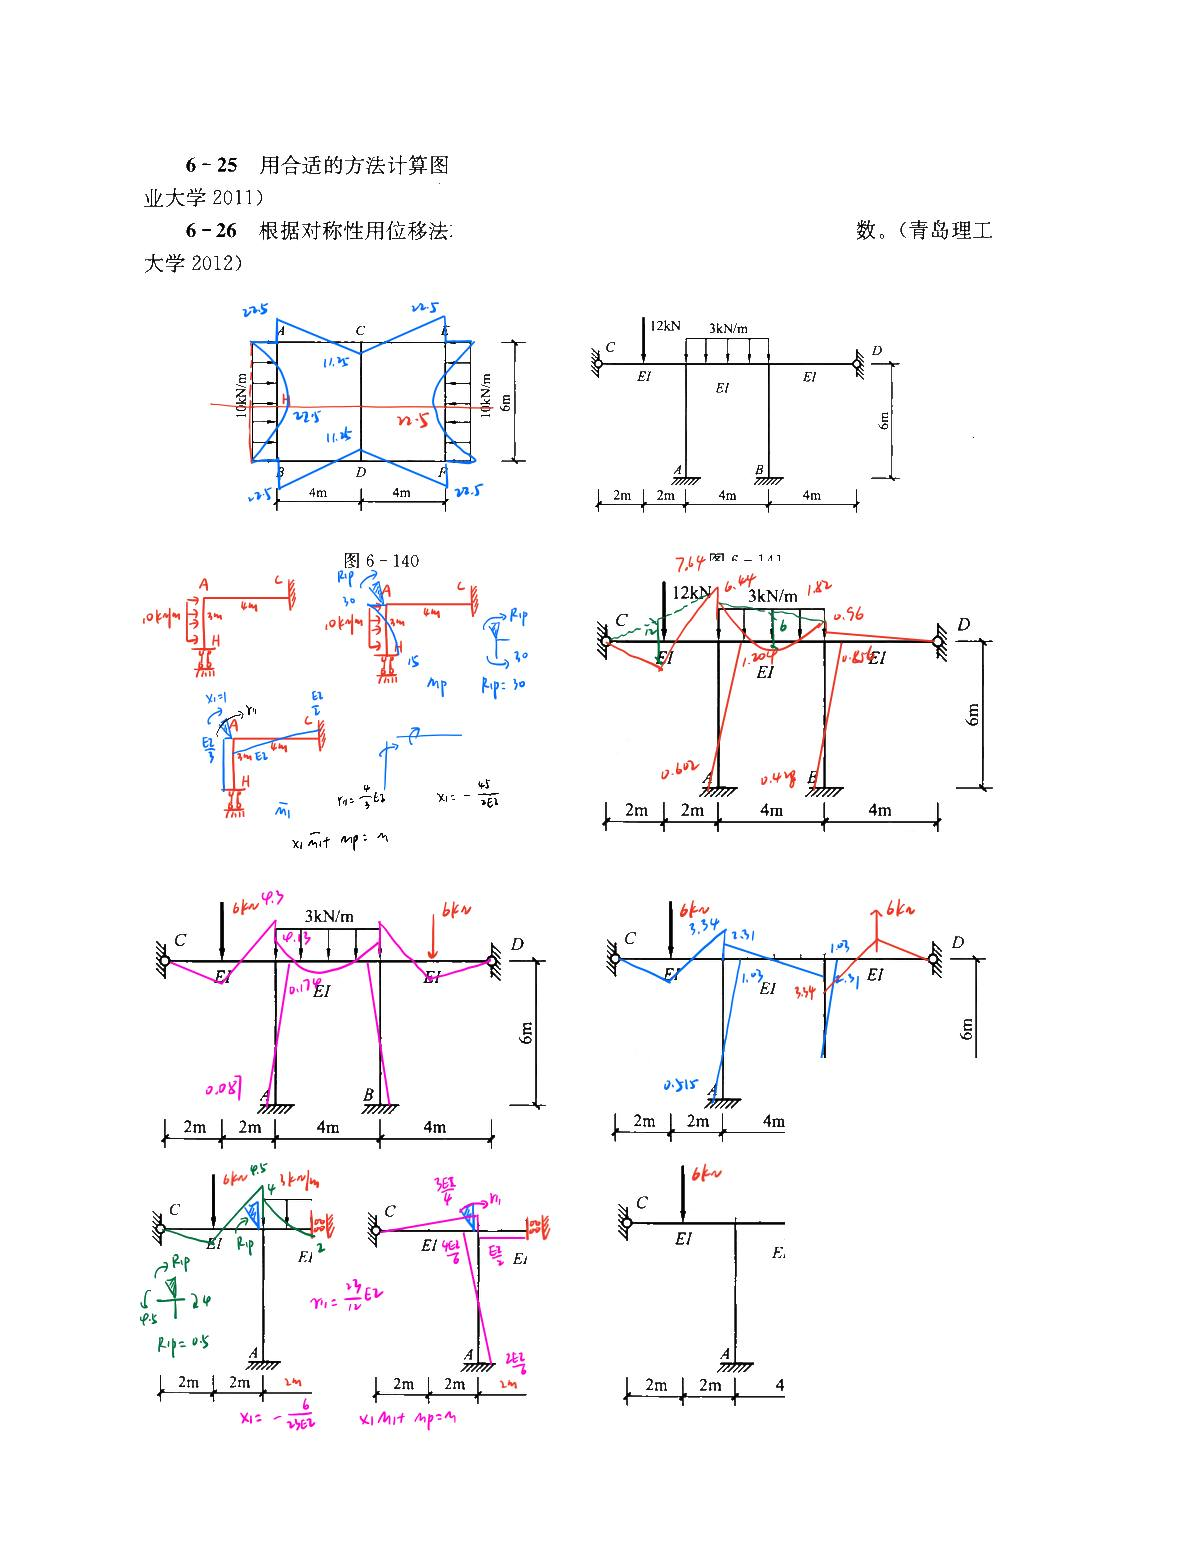
\includegraphics[width=0.92\textwidth]{figures/src31_p015.jpg}
\caption{【第11次作业笔记】 位移法(1) 第 15 页清理图形页}
\end{figure}
\subsection*{第 16 页转写}
iii

ii  

  

in

ii

1蛖

f

f

i 癿

碗

 

t

i

i

i

 

i

i

i

iqoompqi

i.si

Rp

in

二俓

如噐

Xl hit up M
\begin{figure}[H]\centering
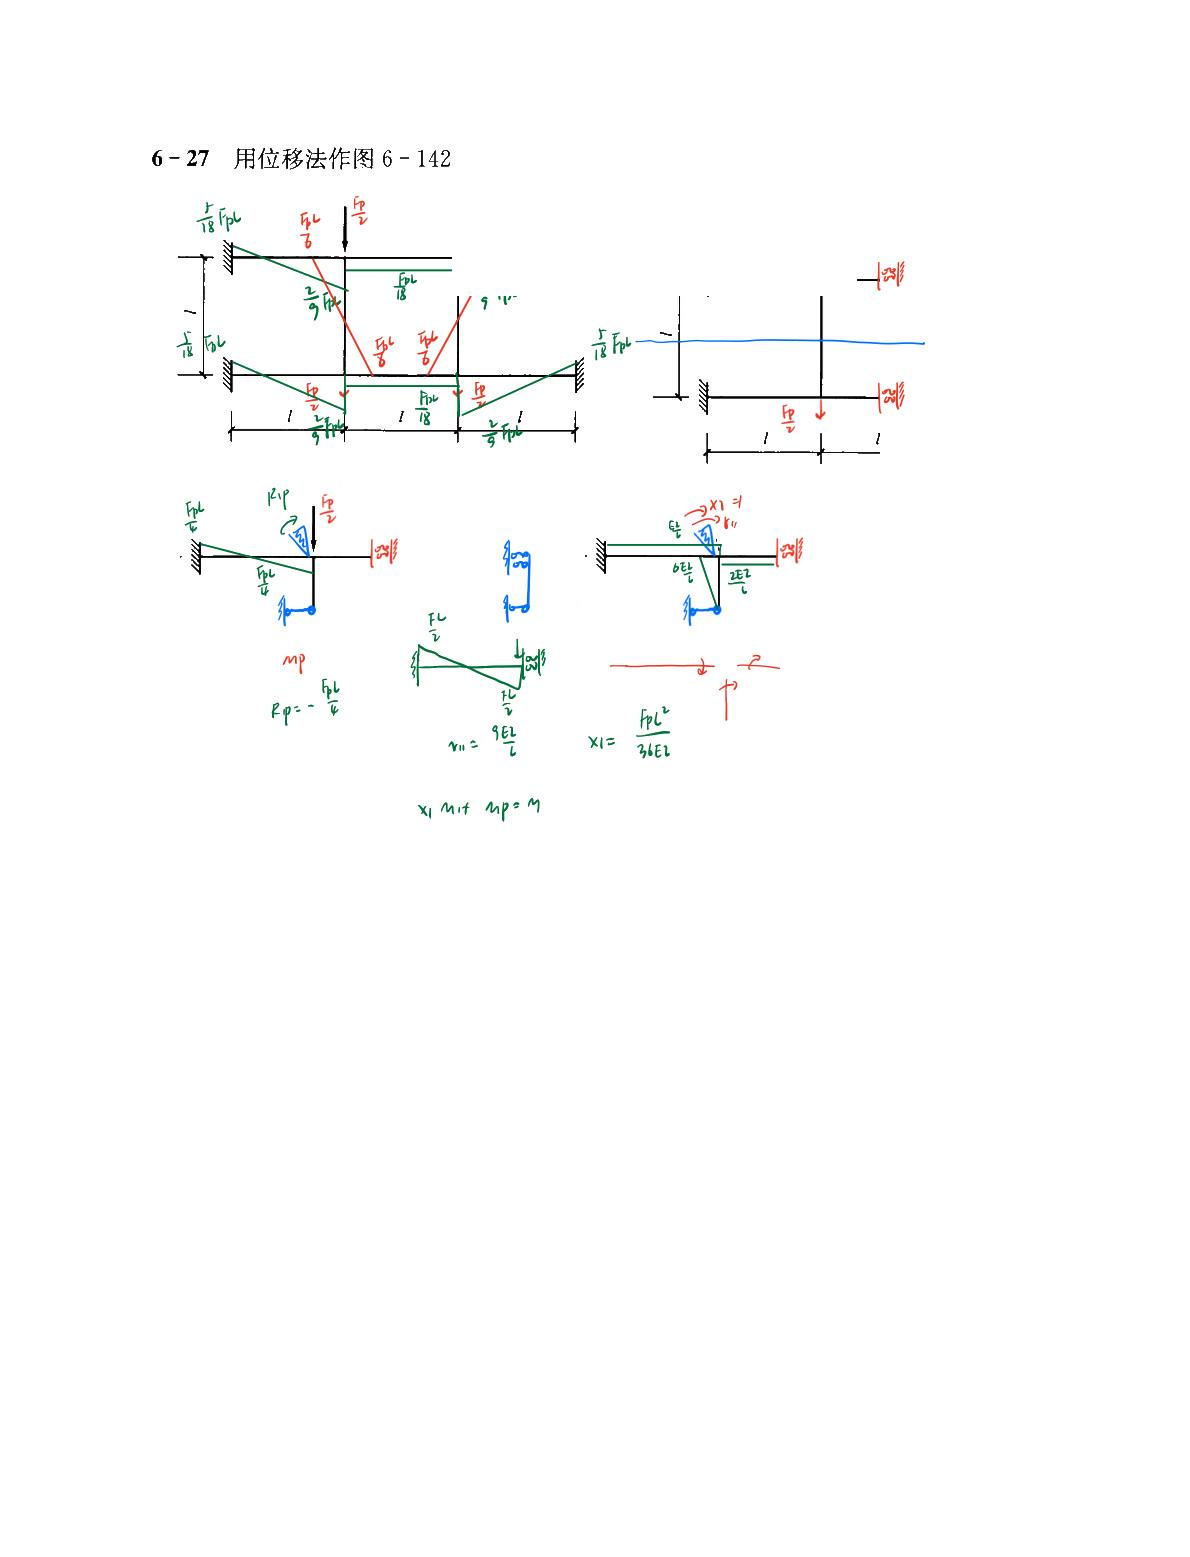
\includegraphics[width=0.92\textwidth]{figures/src31_p016.jpg}
\caption{【第11次作业笔记】 位移法(1) 第 16 页清理图形页}
\end{figure}
\subsection*{第 17 页转写}
6-30用位移法计算图6-145所示结构并作M图，中间支座为弹性支座，其刚度系

数k=5EI/3，EI=常数。（合肥工业大学2009）

Rl+ 元l- Fpx=0

1/2

= + +x"

图6-145

c=d+ X +Xn

367

JRP!

1/2

1/2

Mp

1/2

1/2

199

3E2

XI Mi+ Ximt Mp: M

Yw
\begin{figure}[H]\centering
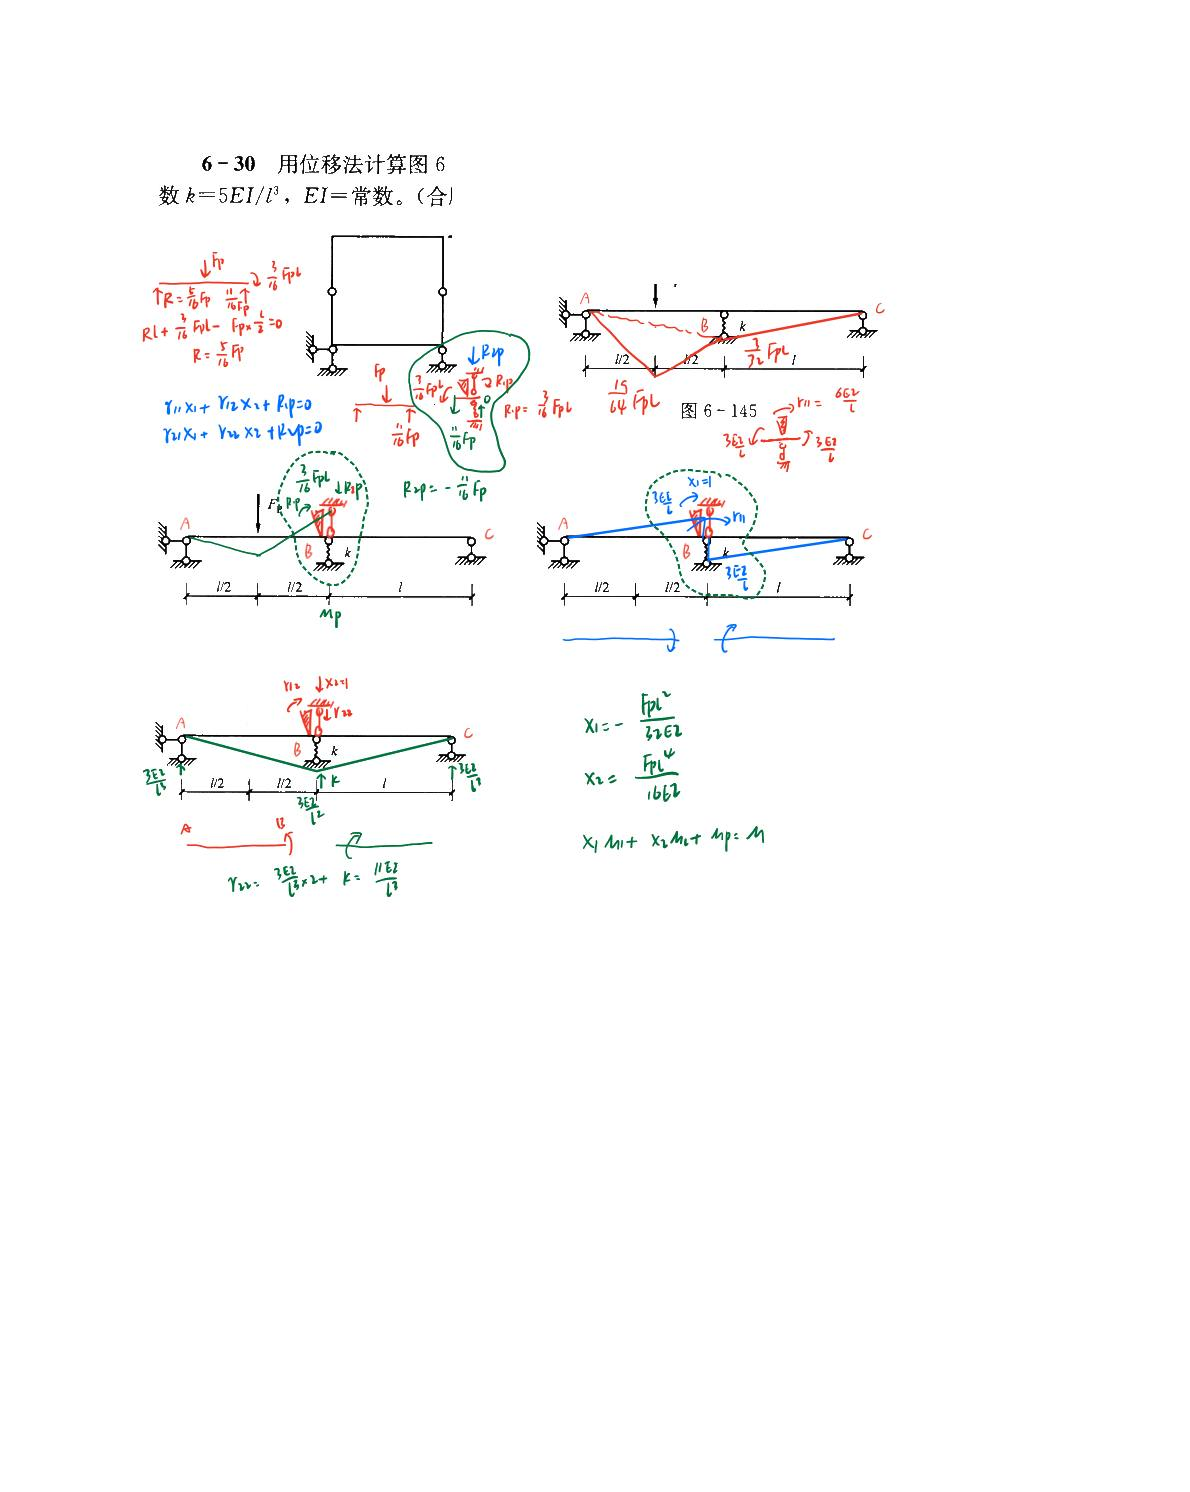
\includegraphics[width=0.92\textwidth]{figures/src31_p017.jpg}
\caption{【第11次作业笔记】 位移法(1) 第 17 页清理图形页}
\end{figure}
\subsection*{第 18 页转写}
7.支座位移和温度改变时的计算

6-31用位移法求解图6-146所示结构的M图（须写出计算过程）。（已知：EI=4.8X

10*kN m ）（东南大学2007）

6-32图6-147所示刚架，B支座产生竖向位移$\triangle$时，试用位移法作弯矩图。（天津

大学2008)

46

21

.02r

6m

6m

图6-146

图6-147

56

16=0.02m

Yn Xit PIc=0

XMI+m=m

0=0.02m

160

31000

2160

Ric=-1 bo

ML

WEL

bx 4.gx 10*+00?

21

21

12E20

131
\begin{figure}[H]\centering
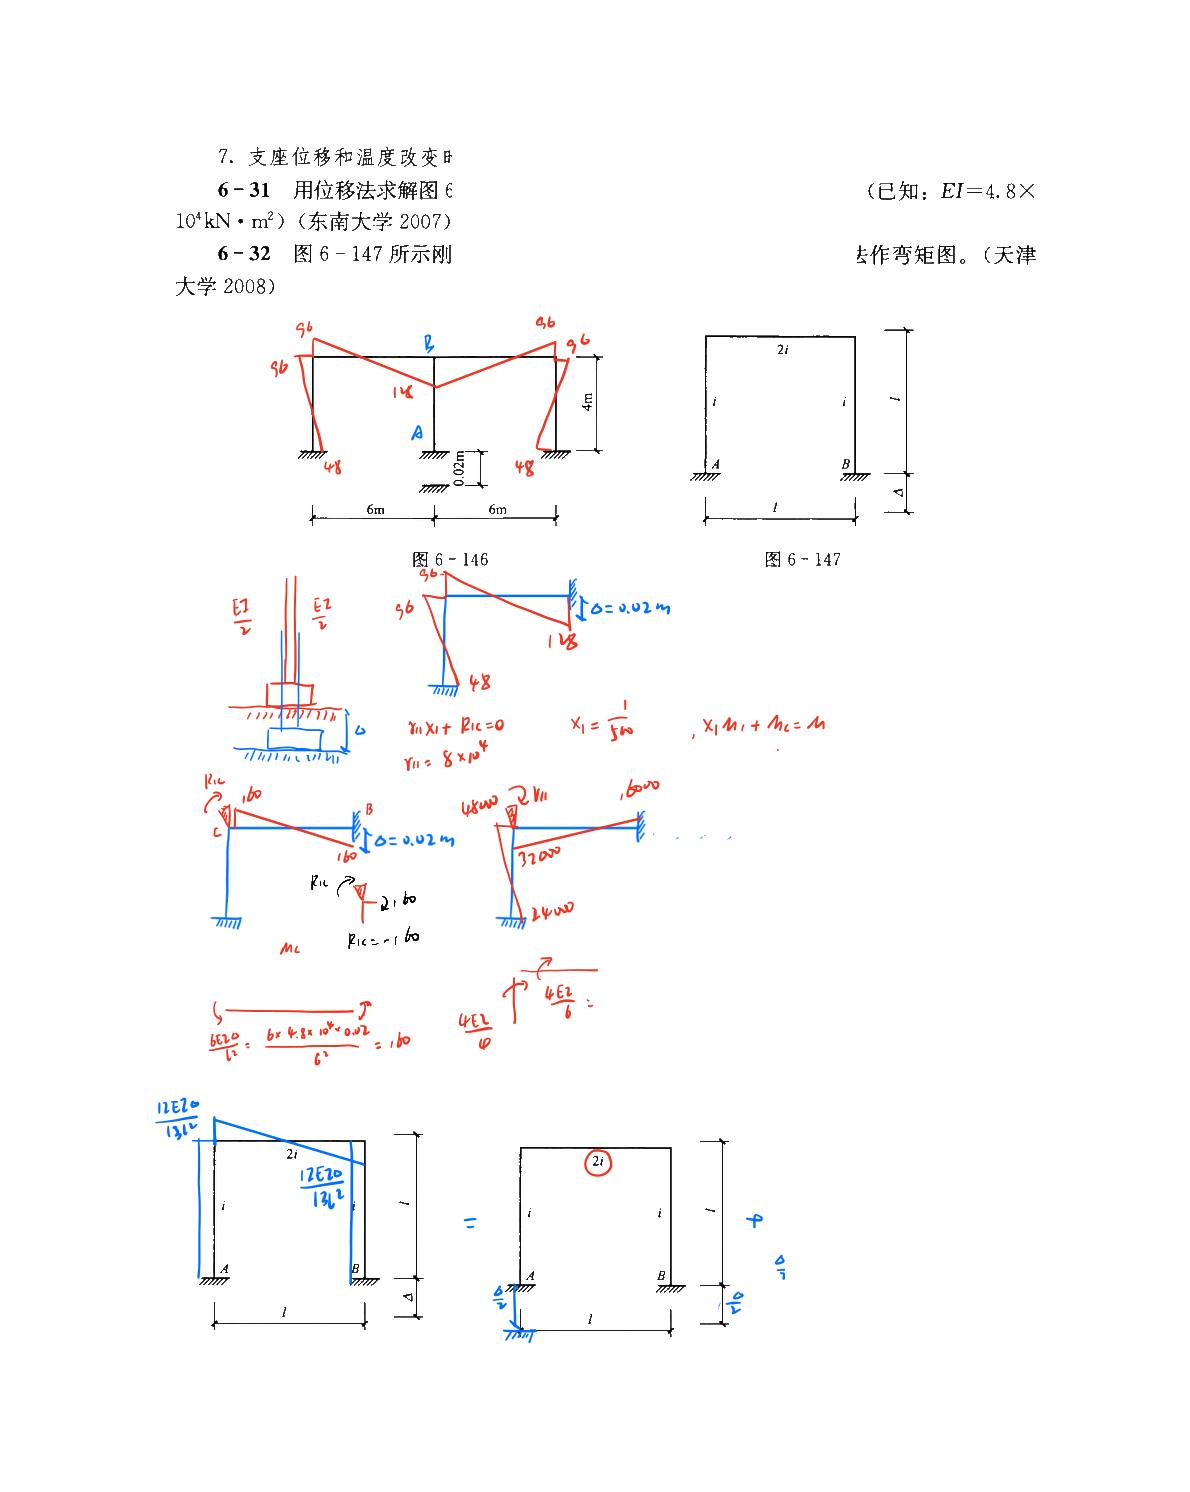
\includegraphics[width=0.92\textwidth]{figures/src31_p018.jpg}
\caption{【第11次作业笔记】 位移法(1) 第 18 页清理图形页}
\end{figure}
\subsection*{第 19 页转写}
巺二2i

升i 

 

4毕4i

n X1

Ria 0

iii

\_

hi 13i

ji

F

in率

幽

Ric一些

mi

Mi

Xi hit

ni

M

ti IE 咔

Bix

华

i

 1

虎
\begin{figure}[H]\centering
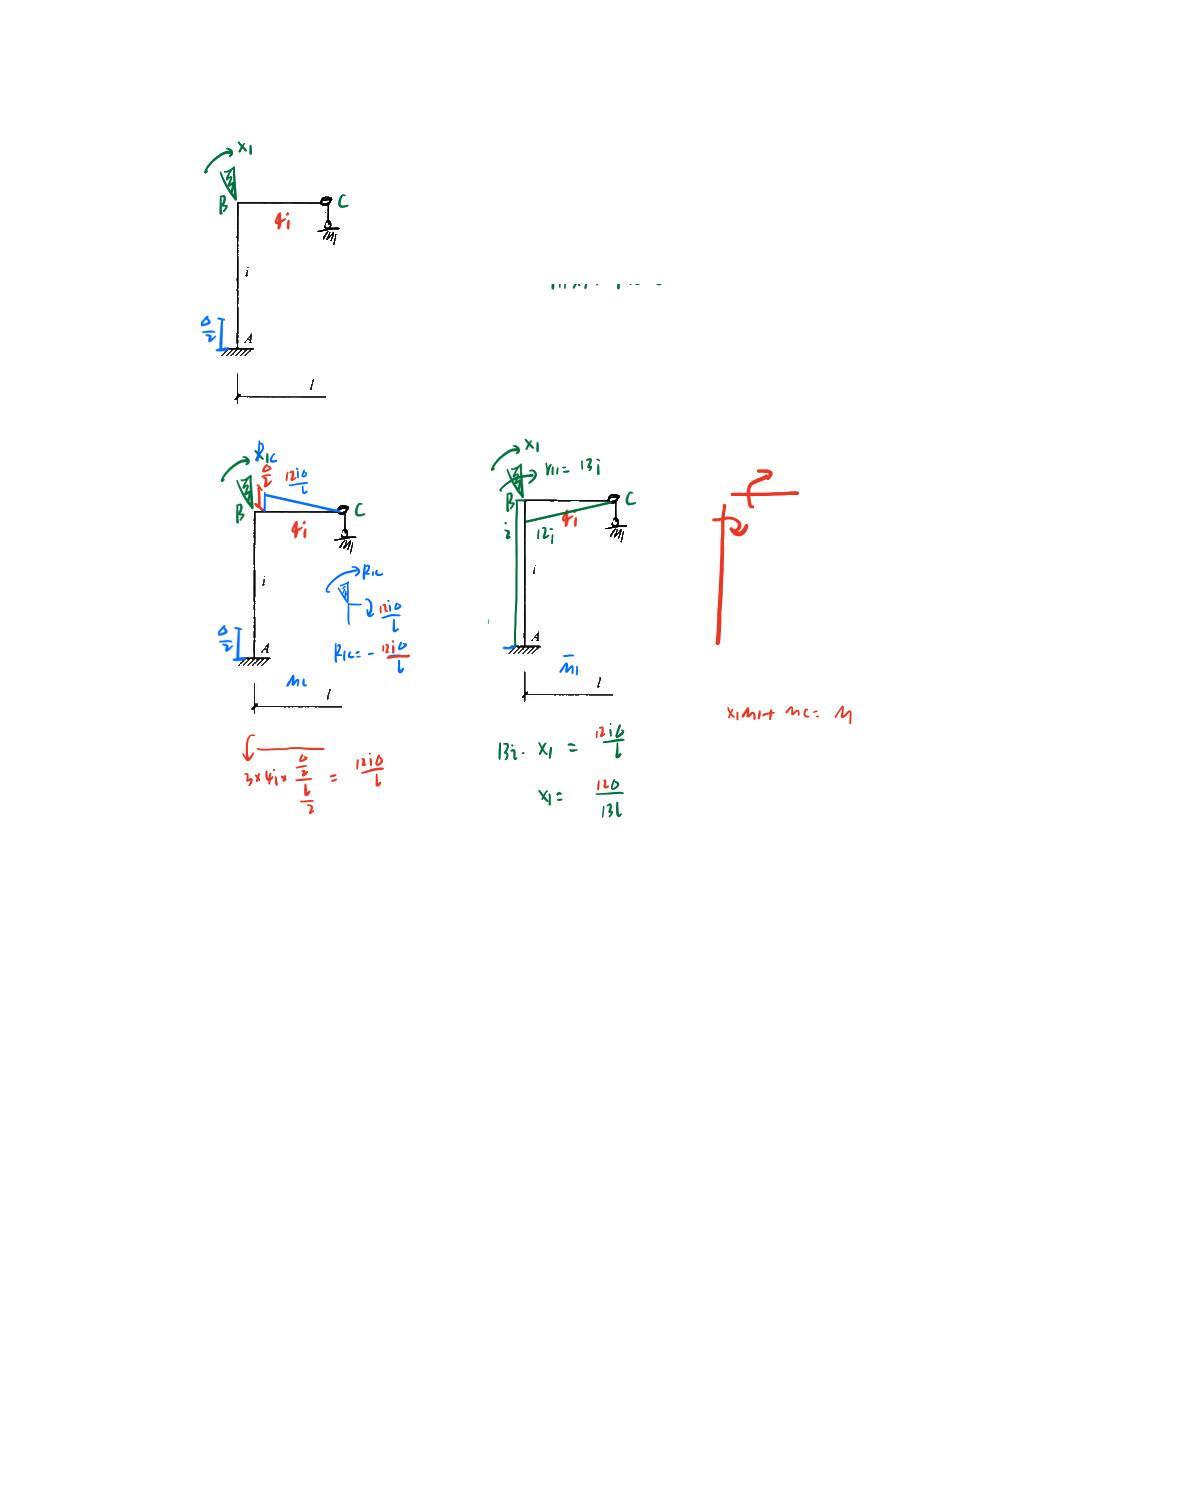
\includegraphics[width=0.92\textwidth]{figures/src31_p019.jpg}
\caption{【第11次作业笔记】 位移法(1) 第 19 页清理图形页}
\end{figure}
\subsection*{第 20 页转写}
8.用位移法求超静定结构的位移

6-33用位移法求解图6-148所示结构未知结点位移。（东南大学2013）

6-34

图6-149所示结构各杆抗弯刚度EI为常数，BC杆受到均布荷载作用，同时D

支座下沉$\triangle$。试求B结点转角

并画出变形图的大致形状。（武汉理工大学2010）

EI

EI

E=080

EI

2ql

Yu Xi+ YnXit Pop=0

Yux+ Yu x2 tRyp=0

图6-148

图0-149

EI

El=00

ER

7993

1191*

TEI

7E2

EI

139
\begin{figure}[H]\centering
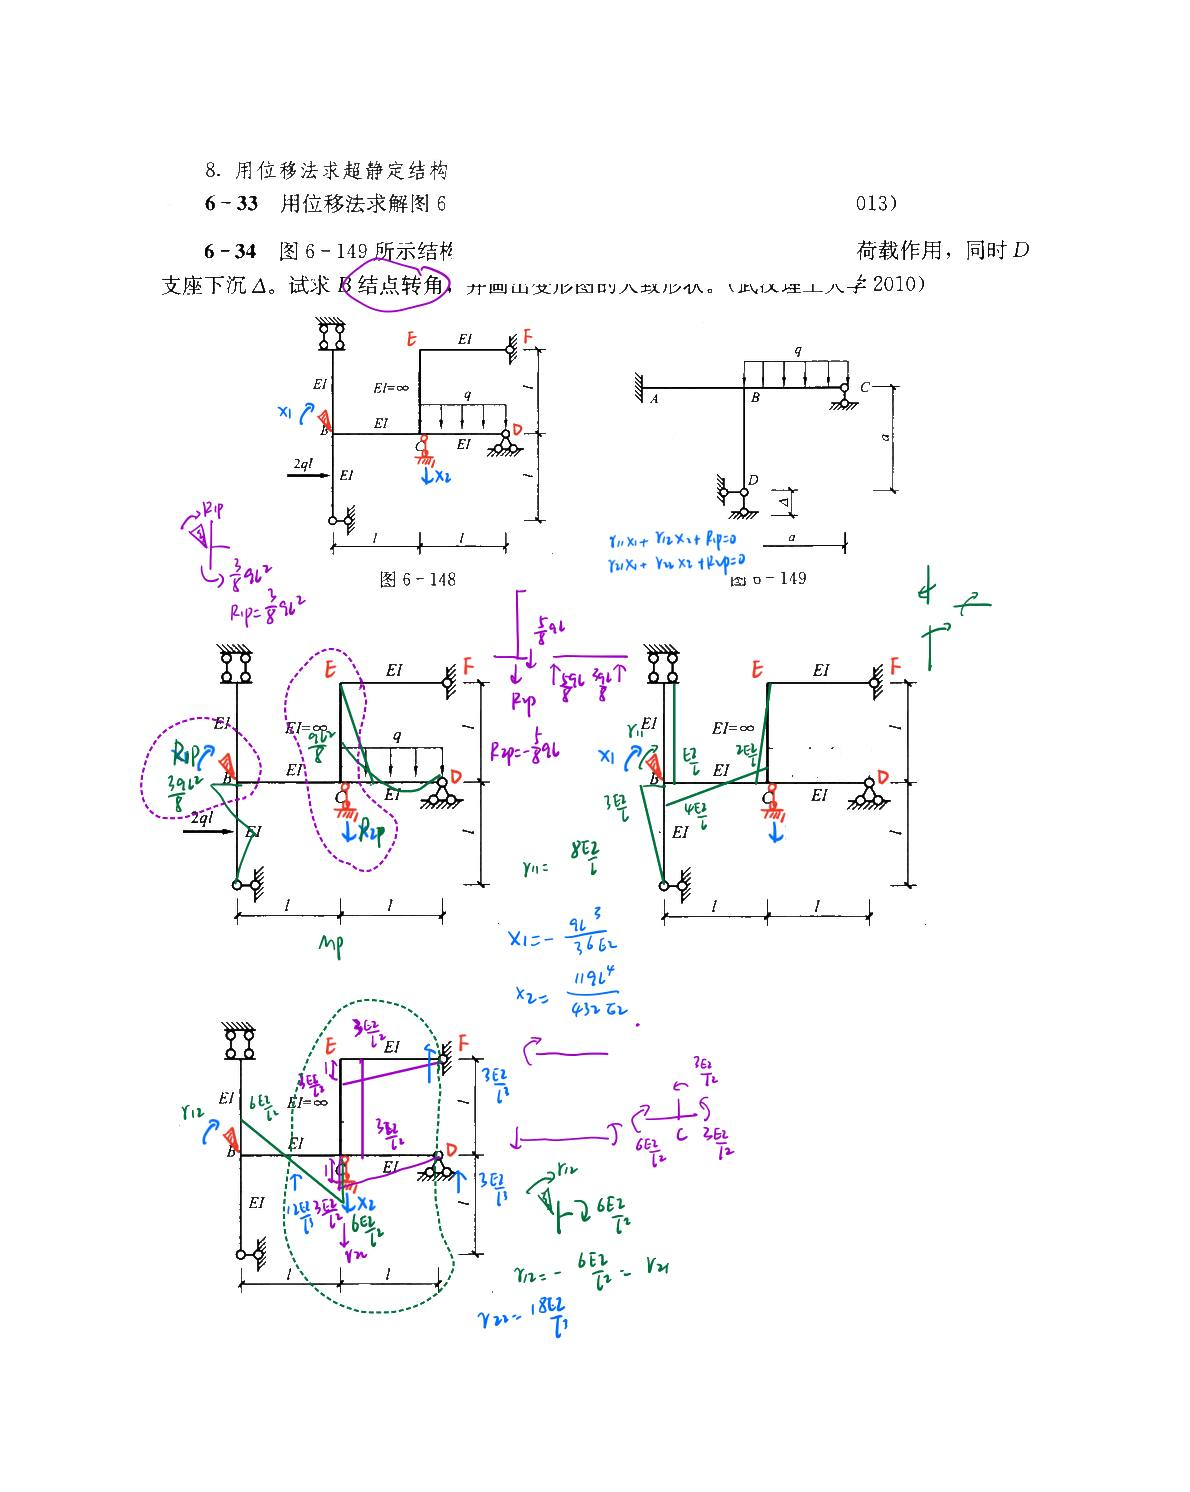
\includegraphics[width=0.92\textwidth]{figures/src31_p020.jpg}
\caption{【第11次作业笔记】 位移法(1) 第 20 页清理图形页}
\end{figure}
\subsection*{第 21 页转写}
giga

3巺

巺in

ii

 1

一

雌

号

rn x it Rip 0

13

c

g Rip

 

等

一笇

x

剝 器

 

Rip 8

一辔十舆

Rip

一辔

一 

s1

1

T
\begin{figure}[H]\centering
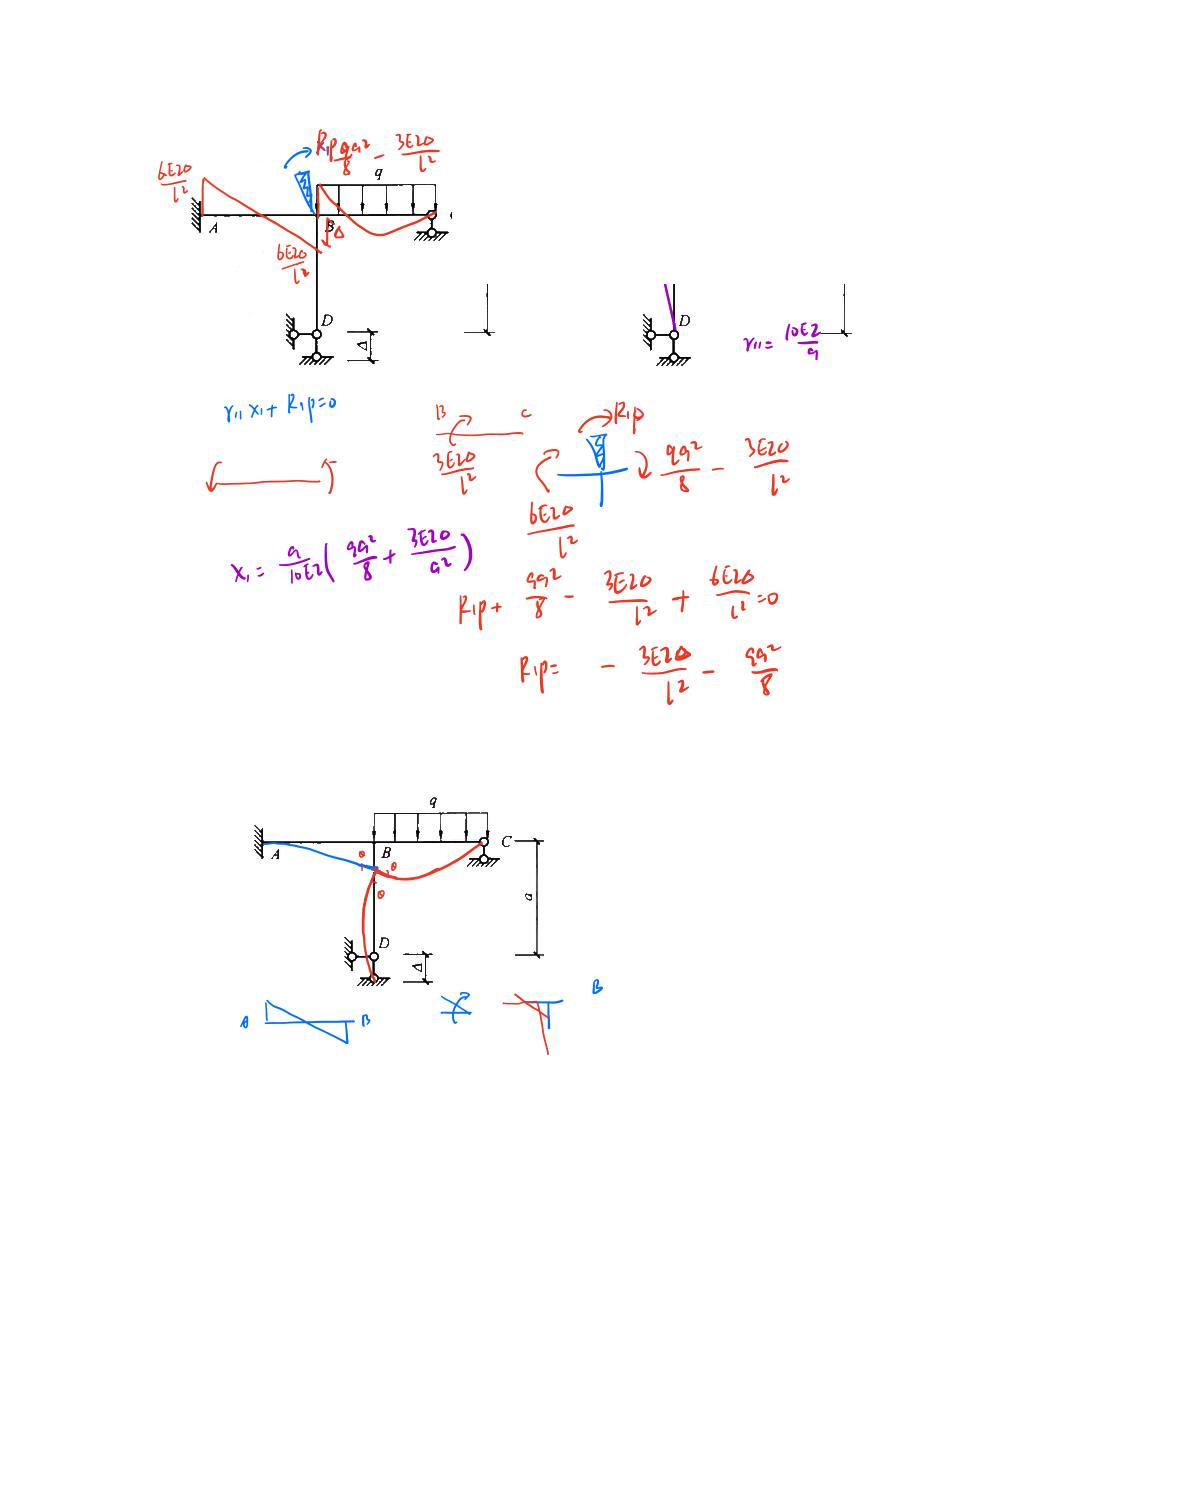
\includegraphics[width=0.92\textwidth]{figures/src31_p021.jpg}
\caption{【第11次作业笔记】 位移法(1) 第 21 页清理图形页}
\end{figure}
